\documentclass[12pt, a4paper, uplatex]{jsbook}
\usepackage{listings,jlisting}
\usepackage{url}
\usepackage{graphicx}
\usepackage[dvipdfmx]{color}
\usepackage{pxrubrica}
\usepackage{here}
\usepackage[dvipsnames]{xcolor}
\lstset{
basicstyle={\ttfamily},
identifierstyle={\small},
commentstyle={\color{OliveGreen}},
keywordstyle={\small\bfseries\color{RedViolet}},
ndkeywordstyle={\small},
stringstyle={\small\ttfamily\color{red}},
frame={tb},
breaklines=true,
columns=[l]{fullflexible},
numbers=left,
xrightmargin=0zw,
xleftmargin=3zw,
numberstyle={\scriptsize},
stepnumber=1,
numbersep=1zw,
lineskip=-0.5ex
}
\renewcommand{\familydefault}{\sfdefault}
\title{テトリス on Pygame}
\author{Swimmy高田馬場校}
\begin{document}
\maketitle
\tableofcontents
\chapter{はじめに}
これから学ぶオブジェクト指向は本来大学の専門科目にあたります。
今も活発に研究が行われている分野ですし、今後10年で大きく変わる可能性もあります。
この本でおすすめしていることも、将来的には\ruby[g]{アンチパターン}{やってはいけない設計}と言われているかもしれません。
今自分はプログラミング言語の最前線を学んでいるんだなあと思って楽しんでくれれば嬉しいです。

\chapter{今まで通りに作る}
\section{いつも通り作ってみよう}
ヘビゲームと同じように、今までのように作ってみましょう。
\lstinputlisting[title={今までのような作り方}, language=Python]{chapter2/tetris.py}
\newpage
\subsubsection{実行結果}
ここまでできたら、次の章に進んでください。実行結果も載せてあるので比べてみてください。
\begin{figure}[h]
  \centering
  % 824x1600
  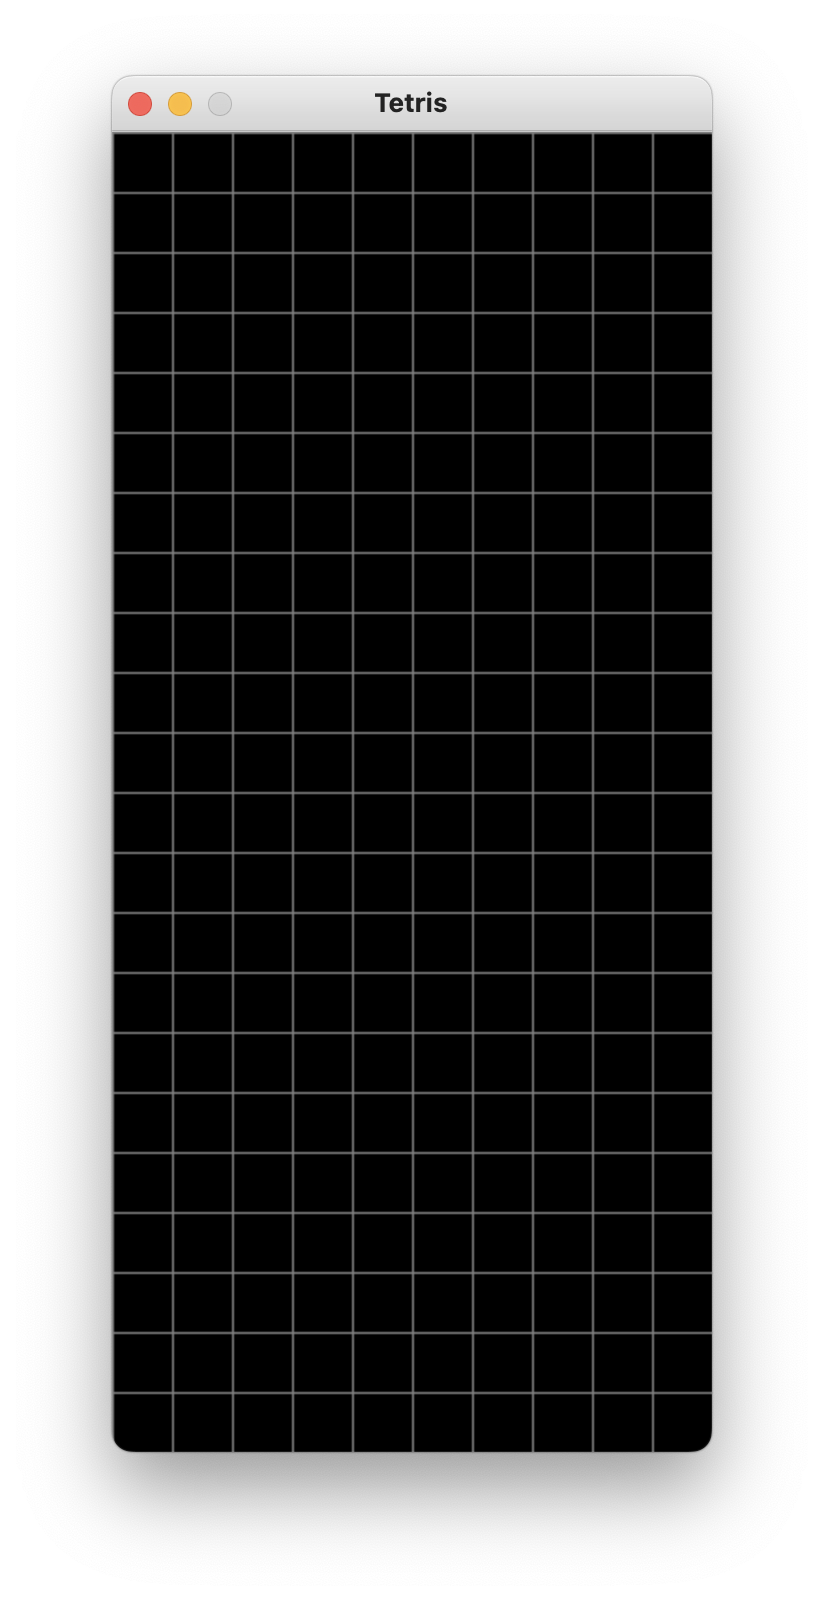
\includegraphics[height=15cm, natwidth=824,natheight=1600]{images/TetrisCH1_1.png}
  \caption{テトリスの実行結果}
\end{figure}

\chapter{オブジェクト指向プログラミングへ}\label{ch:3}
\section{オブジェクト指向プログラミング}
\subsubsection{プログラミング言語界の主人公的存在、オブジェクト指向}
今まで私たちは「変数」、「関数」を用いてプログラムを作ってきました。
\begin{lstlisting}[caption=復習,label=sample, language=Python]
# 変数の作り方
名前 = "ATAI"

# 関数の作り方
def 関数名():
    # その時にすることを書く
    print("こんにちはよいお日和ですね")
\end{lstlisting}
変数はデータに名前をつけることで、関数は処理に名前をつけることでした\footnote{厳密には、変数とはデータの領域に名前をつけることです。}。
オブジェクト指向プログラミングは主に「クラス」という「プログラムそのものに名前をつけたもの」を構成することで
プログラムを作ります。クラスは「変数」と「関数」を持つことができます。つまり、どんなPythonファイルも一つのクラスにまとめることができます。
\section{クラスの作り方}
\subsection{クラスの作り方}
クラスは以下のように作ります。Pythonファイルの中で何個でも作ることができます
\footnote{しかし、みやすさの観点からクラスは1ファイルにつき2〜3個までにする人もいます。}。
\newpage
\begin{lstlisting}[caption=クラスの作り方,label=sample, language=Python]
class クラス名:
    ...
\end{lstlisting}
クラス名は作りたいクラスに応じて変えてください。...は省略しているわけではなく、
「後で書きます」というちゃんとしたPythonのプログラムです。

\subsection{クラスを変数に入れる}
クラスは設計図のようなもので、実際に使うには\textbf{作って変数に入れる}必要があります
\footnote{このような変数のことをインスタンスと呼んだりします。Pythonの場合、全ての変数は何かのインスタンスになるらしいです。}。
\begin{lstlisting}[caption=クラスを変数に入れる,label=sample, language=Python]
変数名 = クラス名()
\end{lstlisting}
\textbf{「クラスを作る」とは「クラス名()」と書くこと}です。作ったクラスは変数に入れないと
次の行には捨てられています
\footnote{捨てられていないこともあります。
  PythonはARCと世代別GCの二種類を持っているらしく、クラスに循環参照がある場合はGCにより時間差で捨てられます}。
なので、大体の場合は「変数名=クラス名()」と書くことが多いです。
カッコの中に何が入るかは、クラスによって異なります。後で説明します。

\subsubsection{関数と似てる?}
クラスは関数と似ている部分があります。関数は使う前になるべく関係ないところで「def 関数名():」と書いて「宣言」
\footnote{こういうものだよ、と決めること}しましたね。
\begin{lstlisting}[caption=関数の作り方,label=sample, language=Python]
def 関数名():
  # 呼ばれた時にすることを書く
  ...
\end{lstlisting}
実際に使うときは、その場所で「関数名()」と書きましたね。
\begin{lstlisting}[caption=関数の呼び出し方,label=sample]
関数名() # 「呼ばれた時にすること」が実行される
\end{lstlisting}
カッコの中には何かが入ったり入らなかったりしますが、関数を使うときは「関数名()」と書きました。
似てますよね。プログラムが複雑になったときに
宣言と使う場所を分離することでプログラムをみやすくするという考え方です。

\section{クラスの中に変数を作る}
\subsection{クラスの中に変数を作る}
普通の変数の作り方と\textbf{ほぼ}同じです。
\begin{lstlisting}[caption=クラスの中に変数を作る,label=sample, language=Python]
class クラス名:
    def __init__(self):
        self.変数名 = 値
\end{lstlisting}
\_\_init\_\_関数は\textbf{クラスを作って変数に入れるときに自動で呼ばれます}。
変数を作って入れることもできますし、printを書くとクラスをつくるたびに表示されるようにすることもできます。
たとえば、教科書に「Mentorクラスを作って、中にageという変数を作る。ageには最初に20を入れる。」という文章があったら、
\begin{lstlisting}[caption=Mentorクラスの作り方,label=sample, language=Python]
class Mentor:
    def __init__(self):
        self.age = 20
\end{lstlisting}
こう書きましょう。\textbf{変数は一つだけでなく何個でも作れます}\footnote{パソコンの覚えられる量を超えない限り}。
さらに、「nameという変数を作って、先生の名前を入れてみよう」という文章があったら、
\begin{lstlisting}[caption=Mentorクラスの作り方,label=sample, language=Python]
class Mentor:
    def __init__(self):
        self.age = 20
        self.name = "先生の名前を入れる"
\end{lstlisting}
クラスはたくさん書くことで設計の仕方がわかっていくので、何度も書く→増やす→失敗する→改良するを繰り返して慣れていきましょう。

\subsection{クラスの変数の中身がわからない場合}
でも、先生の年齢がいつも20歳なのはちょっと変ですね。先生が常に20歳とは限りません。\textbf{クラスは設計図}なので設計段階ではわからない数値やデータもあります。
変数に入れる値がまだわからない時は、引数にすれば\textbf{実際に作る時まで先延ばし}にすることができます。
\begin{lstlisting}[caption=引数を使う場合,label=sample, language=Python]
class Mentor:
    def __init__(self, age, name):
        self.age = age
        self.name = name
\end{lstlisting}
このように書くことで、Mentorクラスを\textbf{作る時に年齢と名前を指定}することができます。
\begin{lstlisting}[caption=Mentorクラスの作り方,label=sample, language=Python]
# クラスを作る時に、年齢と名前を指定する
mentor1 = Mentor(20, "A先生")
\end{lstlisting}
30歳の先生を作る場合は、
\begin{lstlisting}[caption=Mentorクラスの作り方,label=sample, language=Python]
# クラスを作る時に、年齢と名前を指定する
mentor2 = Mentor(30, "B先生")
\end{lstlisting}
さっきのプログラム2つでは違う変数に同じクラスを作っていましたが、\textbf{クラスは設計図}なので、クラスを一度作っておくと、
別のデータで別の変数に似たデータを入れられます。設計図を元にカスタマイズしながら量産できるということです。
まだ便利さがわからないかもしれませんが、関数の引数とオブジェクト指向は
便利さがわかりづらいランキング1位と2位なのでここは少し我慢してください\footnote{作者の個人の感想です}。

\subsection{クラスの変数の中身を変更する}
クラスの変数の中身を変更するには、以下のように書きます。
\begin{lstlisting}[caption=クラスの変数の中身を変更する,label=sample, language=Python]
  mentor3 = Mentor(40, "C先生")
  mentor3.age = mentor3.age + 1
\end{lstlisting}
このように書くことで、mentor3の年齢を1歳増やすことができます。お誕生日おめでとうございます。
\subsection{クラスの変数を使う}
クラスの変数を使うには、以下のように書きます。
\begin{lstlisting}[caption=クラスの変数を使う,label=sample, language=Python]
  print(mentor3.age)
\end{lstlisting}
このように書くことで、mentor3の年齢を表示することができます
\footnote{このようなインスタンスに対して「.」を使ってアクセスする変数をインスタンス変数といいます。}。
普通の変数と同じように使えますね。変数の集まりがクラスと考える人たちもいます
\footnote{厳密には変数を一つに集める機能はストラクチャというものにもあるので、「クラス=変数の集まり」と覚えるのは不正確かもしれません}。

\newpage
\section{クラスの中に関数を作る}
関数の作り方も普通の関数の作り方と\textbf{ほぼ}同じです。
\begin{lstlisting}[caption=クラスの中に関数を作る,label=sample, language=Python]
class クラス名:
    def 関数名(self):
        ...
\end{lstlisting}
引数にselfというものが入っています。これは実際に使うときには入れないので、
「self, 欲しい引数(なければselfだけ)」と書くと覚えておきましょう
\footnote{selfを書かなくても良い言語もありますし、作者個人はそうすべきだと思うのですが…}。
たとえば、教科書に「Carクラスを作って、runという関数を作る。run関数は「走ります」と表示する」という文章があったら、
\begin{lstlisting}[caption=Carクラスの作り方,label=sample, language=Python]
class Car:
    def run(self):
        print("走ります")
\end{lstlisting}
こう書きましょう。\textbf{関数も何個でも作れます}し、引数を使うこともできます。
\begin{lstlisting}[caption=引数を使う場合,label=sample, language=Python]
class Car:
    def run(self):
        print("走ります")
    def set_speed(self, speed):
        print("時速", speed, "kmで走ります")
\end{lstlisting}
テキストを読んでいて「クラスの中に〜」という文章があってよくわからない場合はこの章に戻ってきてください。
ちなみにCarクラスのrun関数を使うには、
\begin{lstlisting}[caption=Carクラスの使い方,label=sample, language=Python]
car = Car()
car.run()
\end{lstlisting}
と書きます。\textbf{クラスは設計図}なので、一度変数にしないと使えません。
run関数は引数selfがあったので「run(何か)」としなければならない気もしますが、
実際に使うときは「car.run()」と書くだけで大丈夫です。
\footnote{このように、インスタンスに「.」をつけて呼ぶことのできる関数をインスタンスメソッドと呼びます。}

\section{まとめ}
クラスは「変数」と「関数」\footnote{正確にはメソッドと呼ばれます。メソッド=手順、手続き}を中に持つことができます。クラスは設計図のようなもので、
実際に使うには変数に入れる必要があります。変数に入れるときは「変数名=クラス名()」のようにしますが、
クラスによってはカッコの中に何かを入れる必要があります。

\subsubsection{先生と調べよう}
答えがないものもあります。暇な時に調べてみてください。
\begin{itemize}
  \item オブジェクト指向プログラミングの良いところと悪いところは?
  \item Pythonの\_\_init\_\_関数などにある\ruby[g]{self}{自分自身}って何?
  \item Pythonのクラスに名前をつけるときのルールは?
\end{itemize}

\chapter{テトリスでクラスを使おう}
\section{main関数の役割を分担する}
クラスを設計するときは、まずクラスの役割を決めます。
ひとまず、\textbf{盤面を管理する}クラスを作ってみましょう。
どんな機能、変数を持っているかはこちらで決めました\footnote{将来は自分で設計することになります。うまくできないと怒られます。}。
\begin{itemize}
  \item 盤面のブロックサイズを表す変数
  \item 盤面のブロックの状態を表すリスト
  \item 盤面をスクリーンに描画する関数
  \item 盤面のブロックサイズから画面の大きさを計算する関数
\end{itemize}
内容が決まってきたらクラスを作ります。
\section{Boardクラスを定義する}
今回はクラスを別ファイルに書いて、インポートする方法にしてみます。
建築でfunctions.pyとmain.pyに分かれていたのと同じような感じです。
まずはこれだけ作ってみましょう。ファイル名は「tetris.py」とし、以下のように書いてください。
\lstinputlisting[title=teris.py, language=Python]{chapter4/tetris.py}
draw関数がscreenを引数にとっているのは、建築でmcを引数にとっていたのと似ています。
Boardクラスは変数にscreenを持っていないので、画面に書くときは一度\textbf{画面を借りる}必要があります。
試しに4行目の「, screen」を消して実行してみてください。「screen is undefined」みたいなエラーが出るはずです\footnote{ちなみにこの段階ではでないです。試してくれた方はごめんなさい。}。
\section{main関数を書き換える}
\subsection{Boardクラスを使ってmain関数を書く}
ここまで読んだら、main.pyを作ります。
\lstinputlisting[title={main.py}, language=Python]{chapter4/main.py}
main関数が少し短くなったと思います。main関数が今までやっていた「盤面に合わせてブロックを書く→線を引く」という
処理をBoardクラス(とそれが入った変数board)に分担したからです\footnote{ここが大事なのでテキストを読んでいない人はこの文を探してみてね}。
でも、この状態ではまだ動きません。tetris.pyのクラスの中で作った関数がまだ「...」のまま残っていますね。実装しましょう。
\subsection{Boardクラスを実装する}
\lstinputlisting[title={tetris.pyを完成させる}, language=Python]{chapter4/tetris2_2.py}
実行すると、一章と同じように動くはずです。

\subsection{ブロックのサイズを変更できるようにする}
ついでに、ブロックのサイズをmain関数から変更できるようにしましょう。
\lstinputlisting[title={tetris.pyを改造する}, language=Python]{chapter4/tetris2_3.py}
\lstinputlisting[title={main.pyを改造する}, language=Python]{chapter4/main2.py}
「{board = Board(tile\_size=30)}」を変えることで、一マスのサイズを変更できます。
ここまでできたら完璧です。

\subsubsection{先生と考えよう}
どちらも正解がないので、暇な時に考えてみてください。
\begin{itemize}
  \item Boardクラスの中にscreenを作らなかったのはなぜ?
  \item main関数の残された役割は?
\end{itemize}

\newpage
\section{クラスの設計を練習する}
\subsection{練習問題1}
まずは以下のプログラムを動かしてみましょう。その後、クラスを使って書き換えてみてください。
\lstinputlisting[title={練習問題1}, language=Python]{chapter4/bank_no_class.py}
このwhile True:では、入力、コマンド確認、残高確認、出力の機能がすべて混ざっています。どういうふうに分離するといいでしょうか?
\newpage
\subsubsection{例}
\lstinputlisting[title={練習問題1の解答例}, language=Python]{chapter4/bank.py}
残高が足りているか確認するのは口座の役割に分担しました。また、残高と名前は別の変数でなく、一つのクラスにまとめました。
同じものに関する情報(変数)は一つのクラスにまとめるのがおすすめです。

\subsection{練習問題2}
まずは以下のプログラムを動かしてみましょう。ゲームになっているので先生と一緒に遊んでみてください。
原因が分かり次第修正します。
\lstinputlisting[title={練習問題2}, language=Python]{chapter4/memory_game_no_class.py}
クラスに分けるとどうなるでしょうか。作るクラスが一つとは限りません
\footnote{2つ以上が正解と言いたいわけではありません。メンターさんは学校の先生と違ってプロじゃないので顔から考えていることがバレやすいです。
  でも、心を読まれて答えを見つけられると微妙な気持ちになります。担当のメンターさんも経験しているかもしれません。}。

\newpage
\subsubsection{例}
\lstinputlisting[title={練習問題2の解答例}, language=Python]{chapter4/memory_game.py}
クラスは複雑になりますが、42〜48行目は短く、分かりやすくなっています。Player()とするだけで入力欄が開くのは便利ですね
\footnote{でも、設計的にはダメな場合もありますので安易にこうしてはいけません}。


\chapter{テトリスのカーソルを作る}
\section{カーソルの設計}
\subsection{カーソルの機能を考える}
カーソルというと、パソコンの矢印のことを思い浮かべるかもしれませんが、現在の
場所を示すものを指します。今回は、テトリスのカーソルを作ります。カーソルはどんな
変数・関数を持つといいでしょうか?今回も教科書の方で決めさせてもらいました。
\begin{itemize}
  \item カーソルの位置を表す変数2つ
  \item カーソルを上下左右に動かす関数
  \item カーソルを描画する関数
\end{itemize}
今回はカーソルのある列は灰色にすることにします。また、カーソルが盤面からはみ出さないように
する機能も上下左右に動かす関数が持つことにします
\footnote{こういう処理をmain関数とかにやらせてしまうと「良くない設計」と言われかねません。
  プログラマの中には「間違った設計」を見るとすごい勢いで設計について語り出す熱心な人もいます。そうした人にも一目置かれるようなプログラマを目指したいですね。}。
\subsection{カーソルの設計について考える}
「カーソルを描画する関数」とありますが、カーソルを描画する方法は2つあります。
\begin{itemize}
  \item カーソルがscreenに対して描画する
  \item カーソルがBoardに指令を出し、Boardがscreenに描画する
\end{itemize}
これらの方法について考えてみましょう。どちらがいいでしょうか?
\newpage
\subsection{設計にけりをつける}
\subsubsection{カーソルがscreenに対して描画する派の主張}
\begin{itemize}
  \item カーソルはBoardとは別の要素なので別に仕事を行うべき
  \item カーソルの情報を盤面に書き込むには、カーソルが盤面の情報にアクセスする必要があり、設計が増える
\end{itemize}
1つ目の要素については個人の自由なのでどちらでもいいですが、
2つ目の要素は考慮する必要があります。

\subsubsection{カーソルがBoardに指令を出し、Boardがscreenに描画する派の主張}
\begin{itemize}
  \item カーソルもBoardの一部
  \item screenに描画するクラスは一つにまとめた方がいい。Cursorもscreenにアクセスするべきではない。
\end{itemize}
実際、カーソルが盤面の一部かどうかについては、\textbf{人によります}。
でも、2つ目の要素は重要です。screenに描画するクラスは一つにまとめた方がいいです。
screenに関してバグがあった時に、screenにアクセスするクラスが一つにまとまっていると
バグの原因を特定しやすくなります。

\subsection{決着}
今回は、このようにします。
\begin{itemize}
  \item カーソルはBoardの一部
  \item カーソルは描画を\textbf{行わない}
\end{itemize}
なので、それぞれのクラスの中身を以下のように変更します。
\subsubsection{Boardクラス}
\begin{itemize}
  \item 盤面のブロックサイズを表す変数
  \item 盤面のブロックの状態を表すリスト
  \item カーソルを表す変数
  \item 盤面, \textbf{カーソル}をスクリーンに描画する関数
  \item 盤面のブロックサイズから画面の大きさを計算する関数
\end{itemize}

\subsubsection{Cursorクラス}
\begin{itemize}
  \item カーソルの位置を表す変数2つ
  \item カーソルを上下左右に動かす関数
\end{itemize}

\section{Cursorクラスを定義する}
\subsection{Cursorクラスを定義する}
tetris.pyにCursorクラスを追加します。
初期状態は中央上側にカーソルがある必要があるので、\_\_init\_\_関数で初期位置を設定します。
\lstinputlisting[title={Cursorクラスを作る}, language=Python]{chapter5/tetris.py}
これだとBoardに直接変数を追加しても良さそうな気もしますが、別の機能は別のクラスに書く、を徹底しましょう。
Boardクラスの\_\_init\_\_関数に「self.cursor = Cursor()」を追加していること、draw関数の最後に
「カーソルの列に対し、BLACKのマスをGRAYにする」処理を入れていることに注意してください。
main関数は変更しなくて大丈夫です。処理を任せることで変更部分を減らすことができるのもオブジェクト指向の特徴です。
実行するとカーソルが出るはずです。

\begin{figure}[h]
  \centering
  % 824x1600
  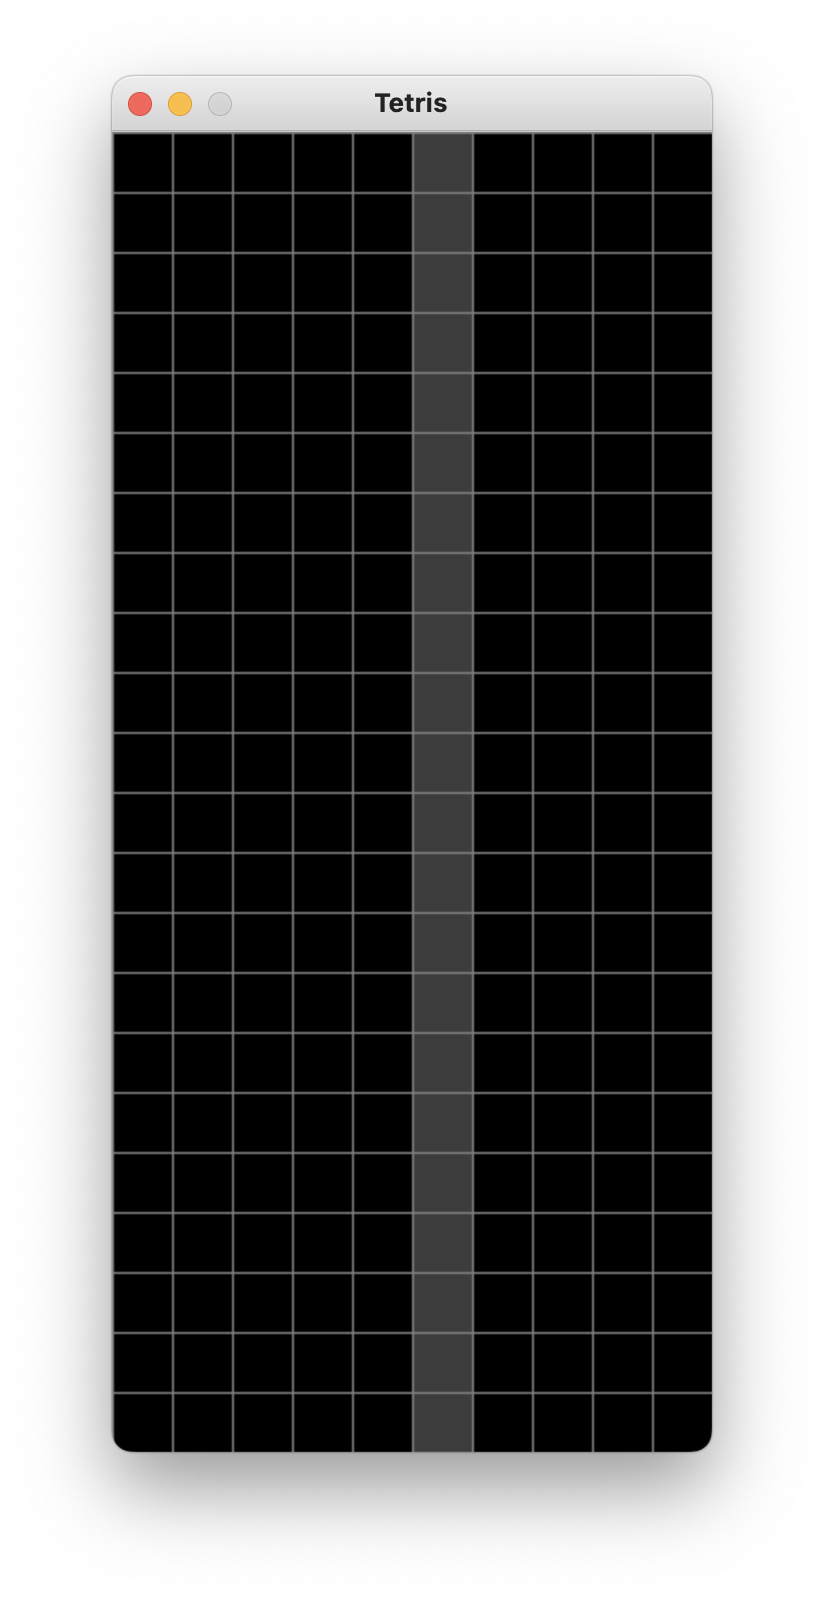
\includegraphics[height=15cm, natwidth=824,natheight=1600]{images/TetrisCH5.png}
  \caption{テトリスの実行結果}
\end{figure}

\section{カーソルを動かす}
\subsection{キー入力を受け取る}
カーソルを動かすには、キー入力を受け取る必要があります。
さて、画面の話でもありましたが、キー入力を受け取る存在も一つにまとめた方がいいです。
どうやって設計すればいいでしょうか?
\begin{itemize}
  \item キー入力を受け取るクラスを作る
  \item main関数にキー入力を受け取る処理を書く
  \item Boardにキー入力を受け取る処理を書く
  \item Cursorにキー入力を受け取る処理を書く
\end{itemize}
このような方法が浮かんできたら、あなたもオブジェクト指向プログラマーの仲間入りです。

キーを受け取るクラスを作る方法はとても「アリ」なんですが、今回はキーの数が少ないのでしません。
Boardにキー入力を受け取る処理を書くと、Boardがキー入力を受け取るという役割が増えてしまいますし、
そもそも盤面に対してキーを打っているわけではないので、これは残念ながら良くないデザインとされます。
Cursorも同様です。今回は「キー入力を受け取るのはmain関数の仕事」とします。後々一時停止や終了などのキーを
作った時に、それをカーソルが受け取るのは不自然ですよね。

\subsection{main関数でキー入力を受け取る}
先ほど決めた通り、main関数でキー入力を受け取ることにします。
\lstinputlisting[title={main関数でキー入力を受け取る}, language=Python]{chapter5/main2.py}
矢印キーでカーソルを動かせるようになりました。pygame.time.wait(100)という見慣れない
文があるかもしれませんが、これは100ミリ秒待つという意味です。mb.sleepと似ていますね。

\section{まとめ}
いろいろ考えた結果、今回はカーソルはBoardの一部ということにして、カーソルの描画はBoardに任せることにしました。
さらに、キー入力を受け取るクラスを作ることも考えましたが、今回はmain関数で受け取ることにしました。
このような設計は先を見据えて行うことが重要ですが、慣れないうちは「とりあえず動くもの」を作ることも大事です
\footnote{今回の設計も正しいとは言い切れません。Boardクラスが「Blob(ブロブ)」状態に陥る兆しがあります。詳しく知りたい人は調べたり聞いてみたりしてください。}。

\subsubsection{先生と考えよう}
キー入力を受け取るクラスを作る場合、どのような設計になるでしょうか?

\chapter{テトリスのブロックを作る}
この章からはプログラムの例を示しません。今までのファイルに追記していく形になります。
\section{ブロックの設計}
\subsection{ブロックの機能を考える}
ブロックは、テトリスの中心的な要素です。ブロックはどんな機能を持つといいでしょうか?
\subsubsection{ブロックの機能}
\begin{itemize}
  \item ブロックを回転させる関数
  \item ブロックを指定した位置に描画する関数
\end{itemize}

\section{ブロックの表示方法を考える}
\subsection{設計}
今回の設計では描画する関数はBoardに任せられています。
しかし、Boardはどんな形のブロックを書くのかわからないのでどうにかしてブロックの情報を
やり取りする必要があります。よって、設計する際にはブロックのクラス、Boardのクラス
両方に機能を加えます。
\subsubsection{設計の案}
\begin{itemize}
  \item Boardが現在保持中のブロックの変数を持つ
  \item Boardはその変数に情報を要求して、その変数は塗らなければいけないマスの座標をリストで返す。これをblock\_info関数とする。
  \item Boardはそのリストをもとに、drawの途中で画面に書き込むことにする
\end{itemize}

図にするとこんな感じです。
\begin{figure}[h]
  \centering
  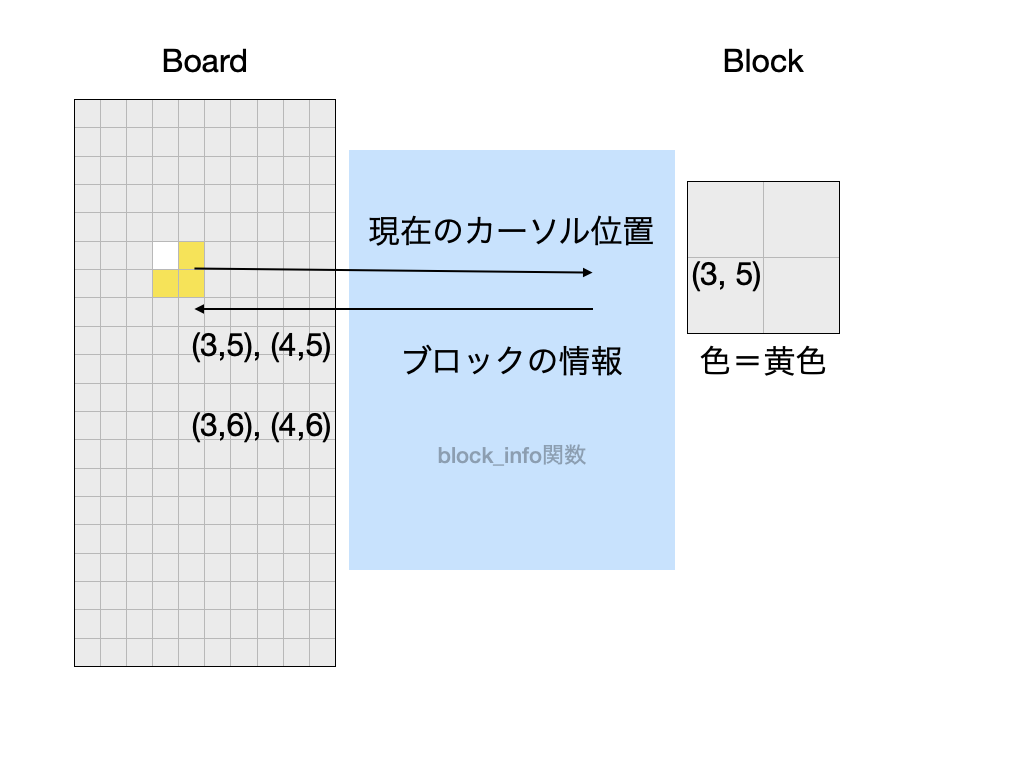
\includegraphics[width=100mm]{images/BoardAndBlock.png}
  \caption{BoardとBlockのやりとり}
\end{figure}

Boardが現在保持中のブロックの変数を持つということなので、Boardクラスに変数を追加します。
最初は何も持っていないので、「動いているブロック」という意味の「moving\_block」にPythonの特別な空を表す「None」を入れておきます。
さらに、ブロックの描画を行う処理をBoardクラスに追加します。画面に書く処理はdraw関数でしたね。
draw関数は現在の盤面を塗る(動かしているブロックは対象外)→カーソルを描く→グリッドを描く、という順番で行われていました。
どこに動かしているブロックを描く処理を入れるか考えてみましょう。
\lstinputlisting[caption={Boardクラスの変更点}, language=Python]{chapter6/ch6_2_1.py}
\texttt{"""..."""}は自分で書いてみましょう。変数の名前を変にしすぎると
先生が助けにくくなります。

\section{ブロックのクラスを定義する}
\subsection{OBlockクラスを定義する}
今回はOブロックを作ります。Oブロックは一番簡単なブロックです。2x2の黄色の正方形です。
最初にこれから作ることにしたのは、回転が必要ないからです。
ブロックにはどのような機能が必要だったか思い出してみます。
\begin{itemize}
  \item ブロックを回転させる関数
  \item 自分の色をもつ変数
  \item ブロックの情報を返す関数
\end{itemize}
\newpage
\lstinputlisting[caption=OBlockクラスの作成, language=Python]{chapter6/ch6_2_2.py}
block\_info関数はカーソルの位置を受け取って、
そこからカーソルの位置、右、下、右下の4つのマスを返します。
Boardはその座標とOBlockの中にあるcolor変数を使って描画します。
rotate関数は今回は作っていませんが、ブロックの種類によっては必要になります。

\section{ブロックを表示させてみる}
\subsection{main関数を変更する}
main関数を変更して、OBlockを動かしてみましょう。
\lstinputlisting[caption={OBlockのテスト}, language=Python]{chapter6/ch6_3_1.py}
うまくいっていれば、Oブロックが動くはずです。
\newpage
\begin{figure}[h]
  \centering
  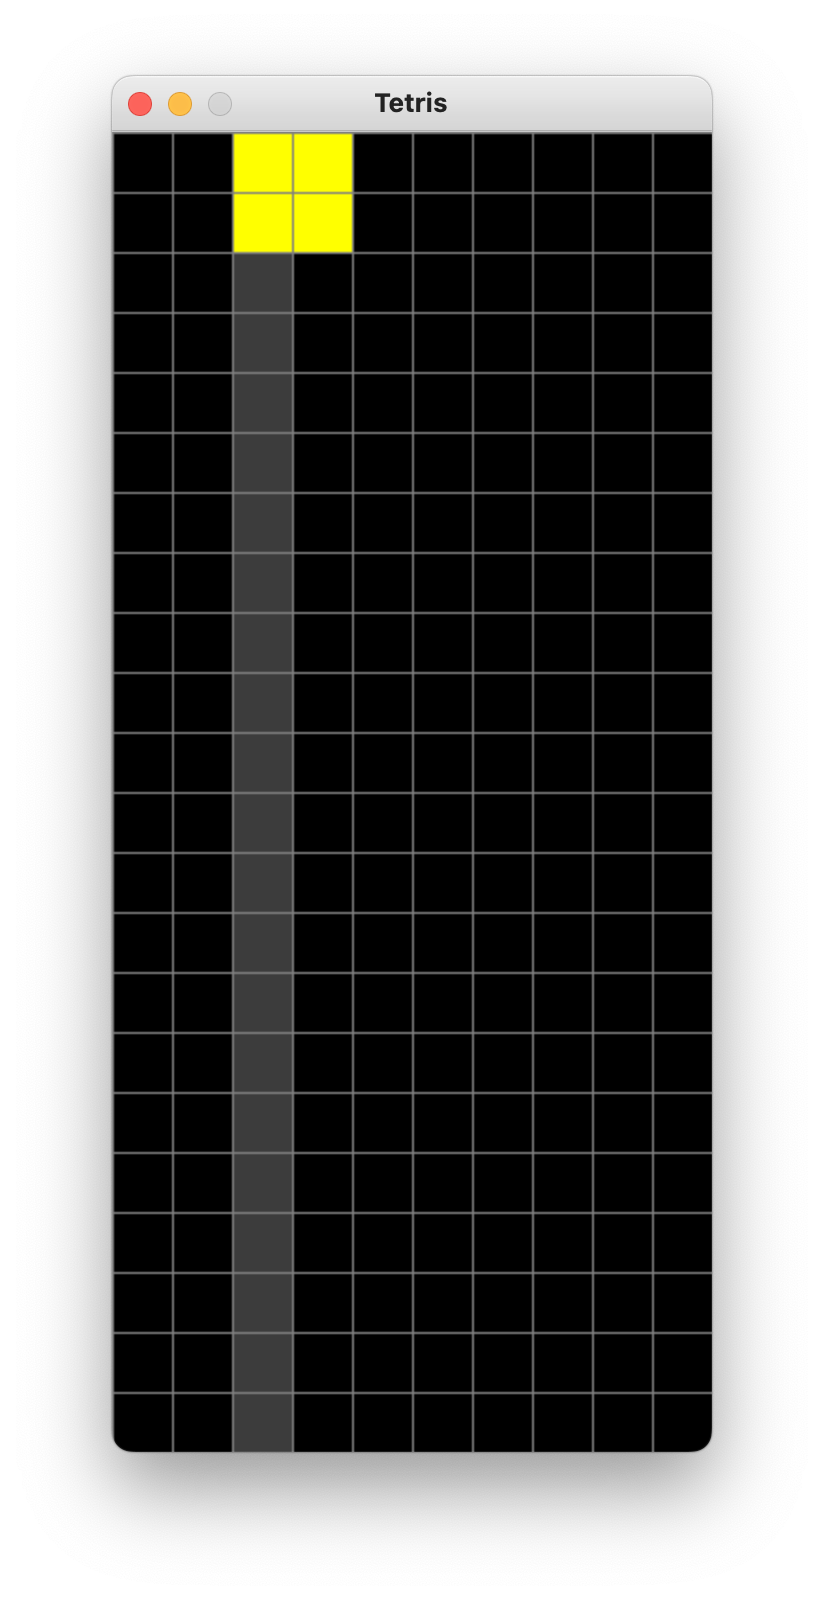
\includegraphics[height=80mm]{images/TetrisCH7.png}
  \caption{テトリスの実行結果}
\end{figure}
\newpage
ここで右端に動いてみましょう。ブロックが半分消えてしまいますね。

\subsection{ブロックの移動範囲を制限する}
この問題を解決するために、ブロックの移動範囲を制限する機能を追加します。
キー入力を受け取ってから動くまでの間に、ブロックが動けるかどうかを判定する処理を入れます。
さて、どこに入れるといいでしょうか?
\subsubsection{設計}
\begin{itemize}
  \item main関数が判定する
  \item Boardが判定する
  \item Cursorが判定する
  \item OBlockが判定する
\end{itemize}
クラスを使う前まではmain関数が判定するのが一般的でした。
しかし、今回はmainには余計な仕事をさせないようにしましょう。
動きを担当するのはCursorの役割です。Cursorにmove\_right関数などを
追加していたはずです。ここを次のように変更することで対処します。
\begin{itemize}
  \item OBlockはCursor, Boardから動けるかどうか計算する
  \item Cursorはその情報をもとに動くかどうか決める
\end{itemize}

\subsection{OBlockクラスを変更する}
OBlockクラスに、動ける範囲を計算する関数を追加します。
\lstinputlisting[caption={OBlockクラスの変更}, language=Python]{chapter6/ch6_3_2.py}
さて、次にカーソルの動きを変更します。
今までは無条件に動いていましたが、一度ブロックを受け取って動けるか
どうかを判定してもらい、動けるなら動くようにします。

\subsection{Cursorクラスを変更する}
\lstinputlisting[caption={Cursorクラスの変更}, language=Python]{chapter6/ch6_3_3.py}
これらの変更が終わると、main.pyにエラーが出ているはずです。
今まではcursor.move\_right()のように書いていましたが、
これからは引数としてboardとblockを渡す必要があるからです。
もちろん、main関数で引数を渡すように変更しても良いのですが、
少し見栄えが悪いので(プログラマとしては見栄えが悪いです)、変更を加えます。
\subsection{Boardクラスを変更する}
今回はカプセル化という方法で、BoardクラスがCursorをカプセルのように閉じ込めて、
Board経由でCursorを操作するようにします。
そこで、Boardクラスにmove\_right関数を追加し、Cursorのmove\_right関数を呼び出すようにします。
\lstinputlisting[caption={Boardクラスの変更}, language=Python]{chapter6/ch6_3_4.py}
\subsection{main関数の変更}
最後に、main関数を変更して、cursorを使うのではなく、boardの移動機能を使うようにします。
\lstinputlisting[caption={main関数の変更}, language=Python]{chapter6/ch6_3_5.py}
これを実行すると、ブロックが右端に行かなくなります。
また、下方向にも消えずに止まるようになります。

\section{まとめ}
今回は、簡単なOBlockを作成しました。Boardクラスにブロックの情報を持たせ、
Boardは適宜OBlockに情報を要求して描画するようにしました。
また、ブロックの移動範囲を制限する機能を追加し、Cursorクラスにその機能を持たせました。
最後に、main関数を変更して、CursorではなくBoardを使ってブロックを動かすようにしました。

\subsubsection{懺悔}
正直にいうとこのテトリスの設計、若干失敗したなあと思っています。
今はBoardがmoving\_blockを持っています。しかし今回の章でいえば、ブロックをCursorの中に持たせるべきでした。
そうであればBoardがCursorをカプセル化する必要もなかった上に設計が簡単になります。
今後ブロックを落とす処理を追加するときを見越してこのような設計にしたのでいいのですが、
果たしてこれが正解だったのか、今後の展開にご期待ください。

\chapter{回転するブロックを作る -- Tブロック}
\section{Tブロック}
今回はTブロックを作ります。Tブロックは、Tの字の形をしています。
Tブロックは、回転が必要なブロックです。回転するためには、ブロックの形を表す変数が必要です。
今回は、ブロックの形を方角と対応させて持つことにしますが、
\textbf{Tブロックの上の横棒が向いている方が方角になる}ようにします。また、カーソルの位置が
Tのくっついているところになるようにします。

\begin{figure}[h]
  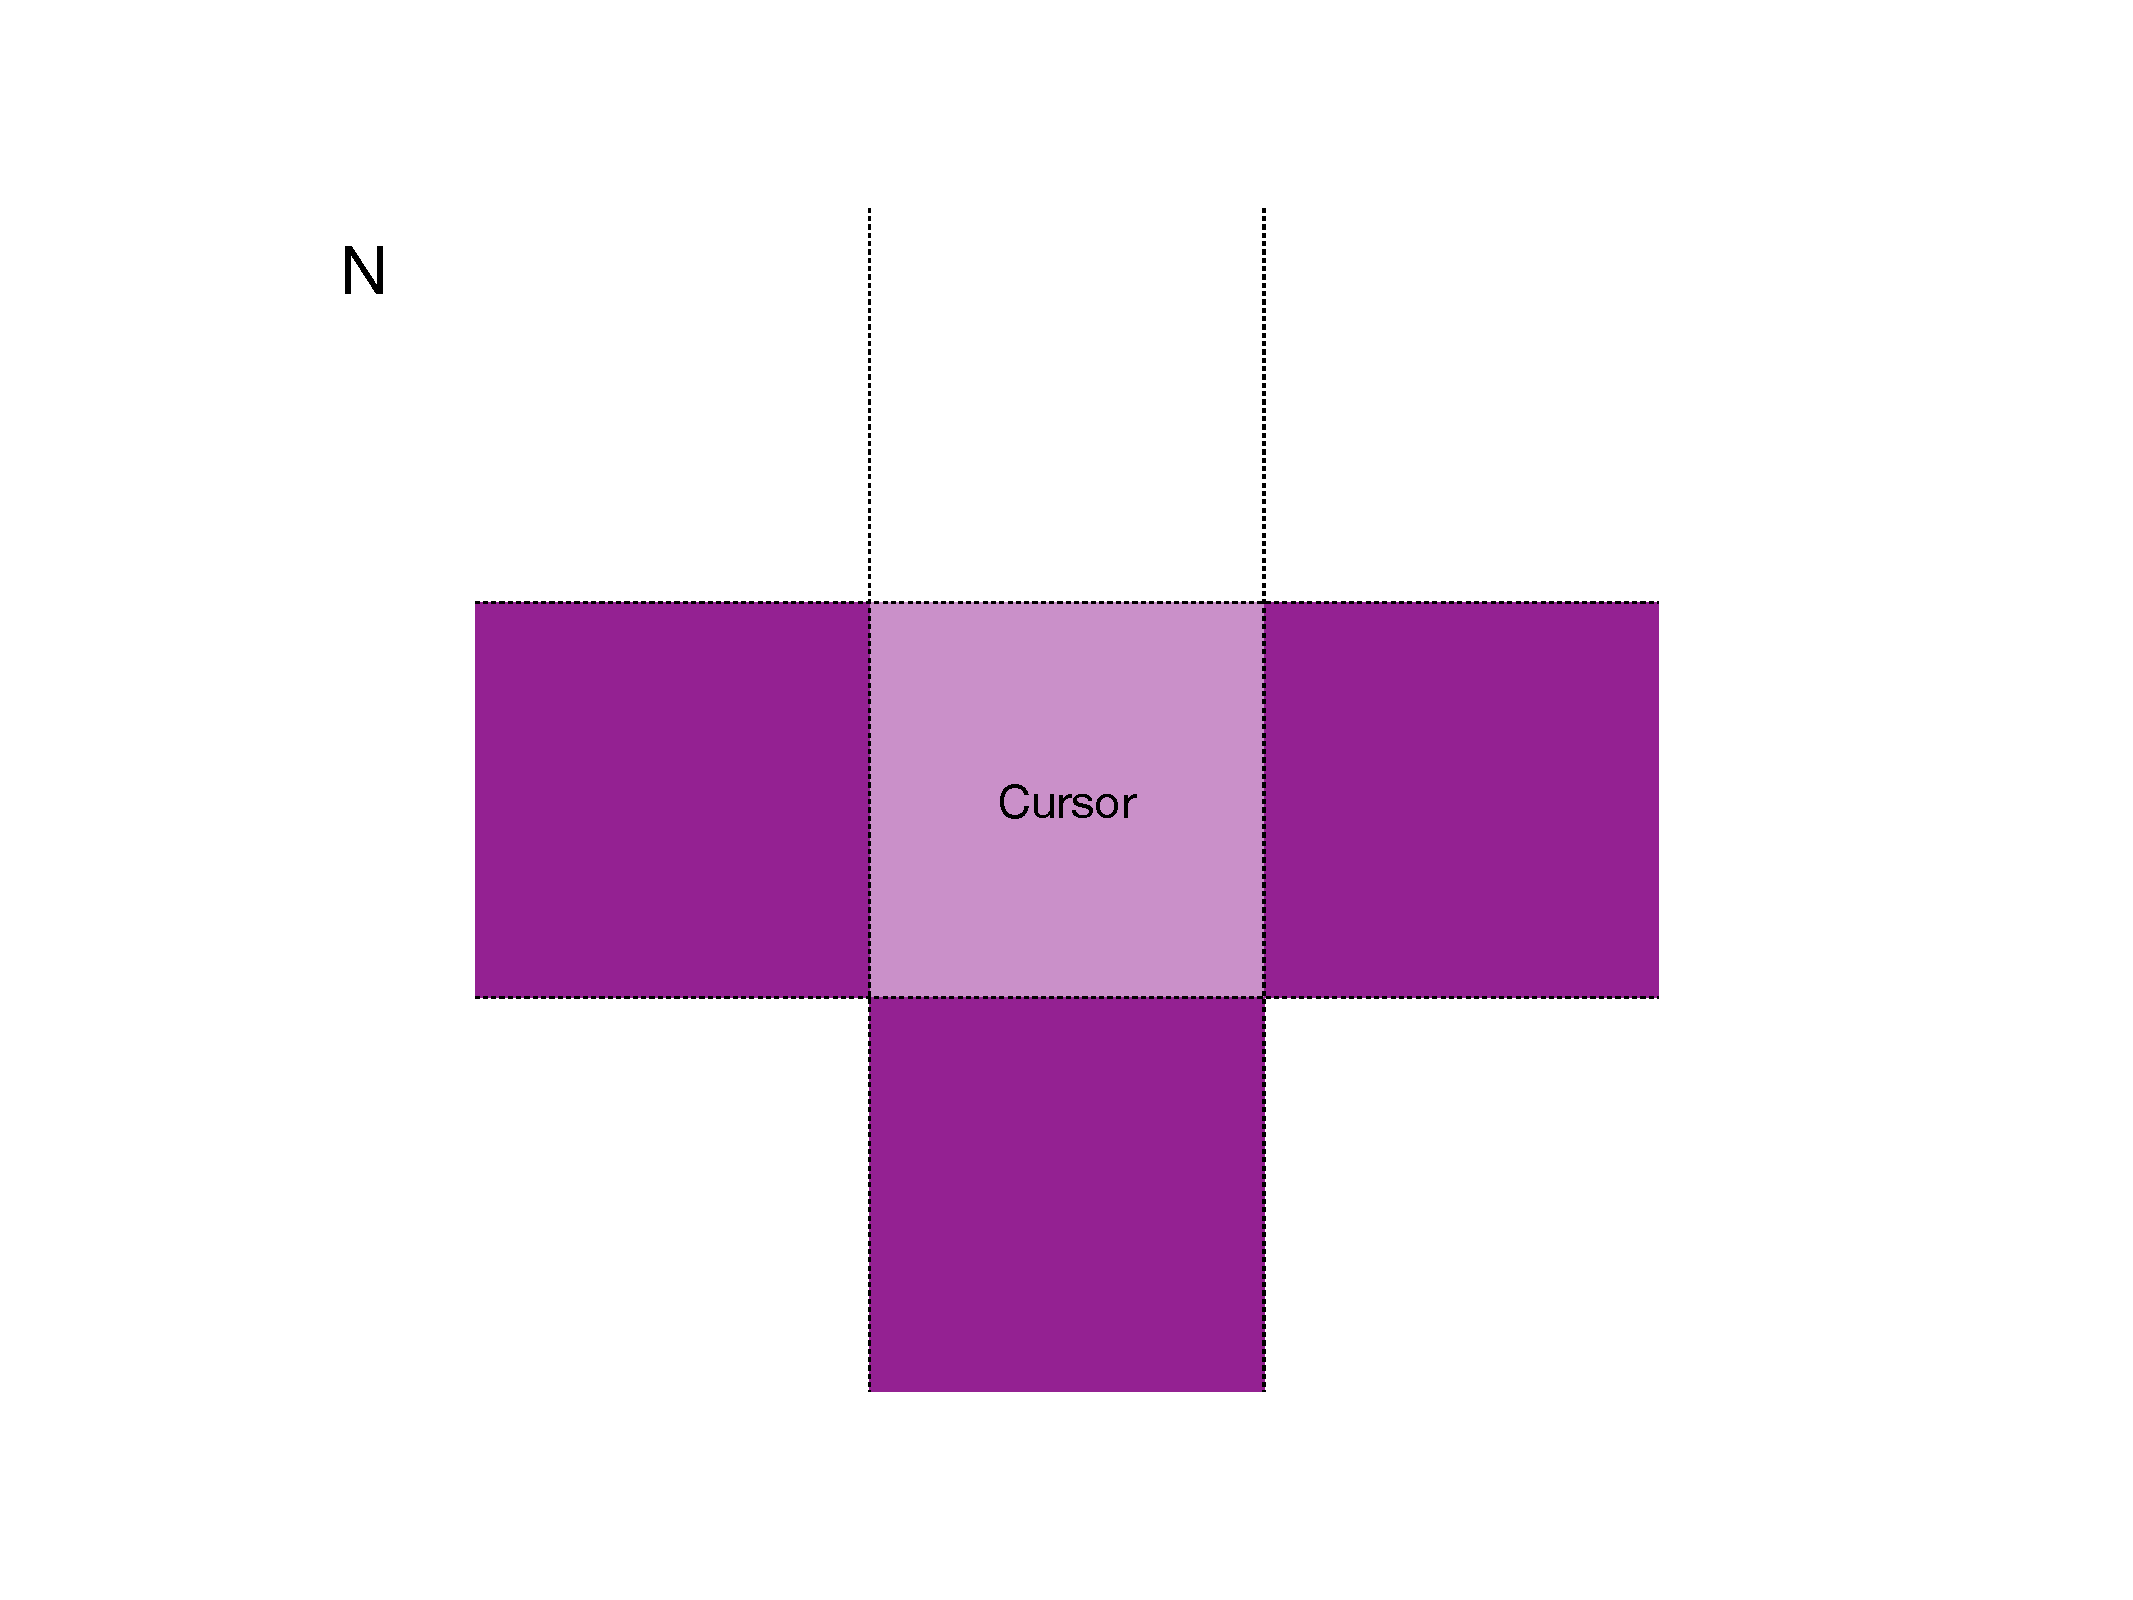
\includegraphics[width=70mm, page=1]{images/Blocks.pdf}
  \includegraphics[width=70mm, page=2]{images/Blocks.pdf}
  \includegraphics[width=70mm, page=3]{images/Blocks.pdf}
  \includegraphics[width=70mm, page=4]{images/Blocks.pdf}
  \caption{Tブロック}
\end{figure}

\newpage
\subsection{Tブロックのプログラム}

\lstinputlisting[caption={Tブロックのプログラム}, language=Python]{chapter7/ch7_1_1.py}

\newpage
\subsubsection{プログラミング豆知識}
回転系、周期系の変数の処理を楽に書きたいときは、それらを0から始まる数字の連番にすることと、
あまりが繰り返すことを利用すると上手く書けます。
\begin{lstlisting}[caption=方角を扱う,language=Python]
N=0
E=1
S=2
W=3
direction = N
direction = (direction + 1) % 4 # directionはE(1)になる
direction = (direction + 1) % 4 # directionはS(2)になる
direction = (direction + 1) % 4 # directionはW(3)になる
direction = (direction + 1) % 4 # directionはN(0)になる、3+1は4だが、4を4で割った余りは0なため
\end{lstlisting}
このように、Nから始まった方角がまたNに戻ってきます。

\subsection{Tブロックの描画}
Tブロックの描画は、Oブロックと同じように行います。
OブロックはBoardにblock\_infoを求められ、その情報をもとに描画していました。
でも、Tブロックもblock\_infoを持っていますから、Oブロックと同じように描画できます。
つまり、\textbf{Boardクラスは変更が必要ありません。オブジェクト指向の利点です。}
違うクラスであっても同じ名前で関数を設計すると、他のクラスから同じように扱えます。
でも中身自体は違うので、それぞれのブロックがそれぞれにあった情報を返すことができるのです。
こういう性質を「ポリモーフィズム/多態性」と言います
\footnote{厳密には違うんですがPythonにポリモーフィズムはあってないようなものなので教えるとしたらこうするしかないんです}。
では、main関数を変更して最初にTブロックを表示してみましょう。
\lstinputlisting[caption={テスト用にTブロックを表示}, language=Python]{chapter7/ch7_2_1.py}
できたら実行しましょう。表示だけで動かすとエラーになります。
\begin{figure}[h]
  \centering
  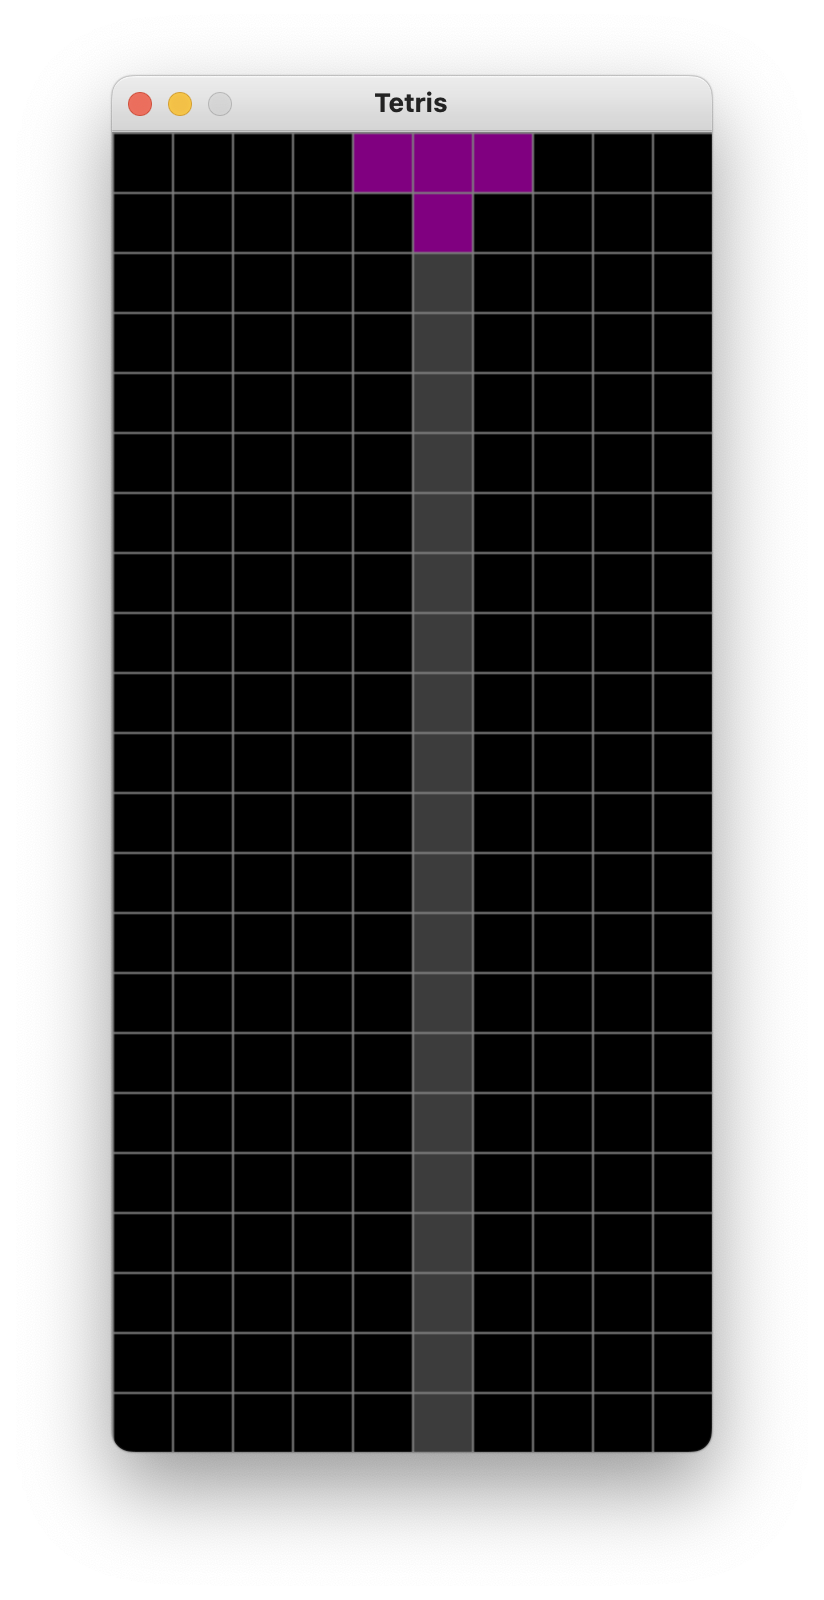
\includegraphics[width=50mm]{images/CH7_2.png}
  \caption{Tブロックの表示}
\end{figure}

\section{Tブロックを動かす}
なぜエラーになったのでしょうか?それは、Tブロックが動けるかどうかを判定する機能がないからです。
Oブロックは動けるかどうかを判定する機能を持っていましたが、Tブロックにはありません。
Boardはそのことを知らずにその関数を呼び出してしまったためエラーになります。
Tブロックにも動けるかどうかを判定する機能を追加しましょう。
\subsection{Tブロックに動けるかどうかを判定する機能を追加する}
TブロックにもOブロックと同じように、動けるかどうかを判定する機能を追加します。
\lstinputlisting[caption={Tブロックに動けるかどうかを判定する機能を追加}, language=Python]{chapter7/ch7_3_1.py}

\subsection{あれ、回転は?}
main関数でキー入力を受け取っていますので、main関数を実行して回転キーを設定しましょう。

\lstinputlisting[caption={main関数で回転する}, language=Python]{chapter7/ch7_4_1.py}
書き終えたら実行してみましょう。ひとまずお疲れ様でした。でも、まだ終わりではありません。
\begin{figure}[h]
  \centering
  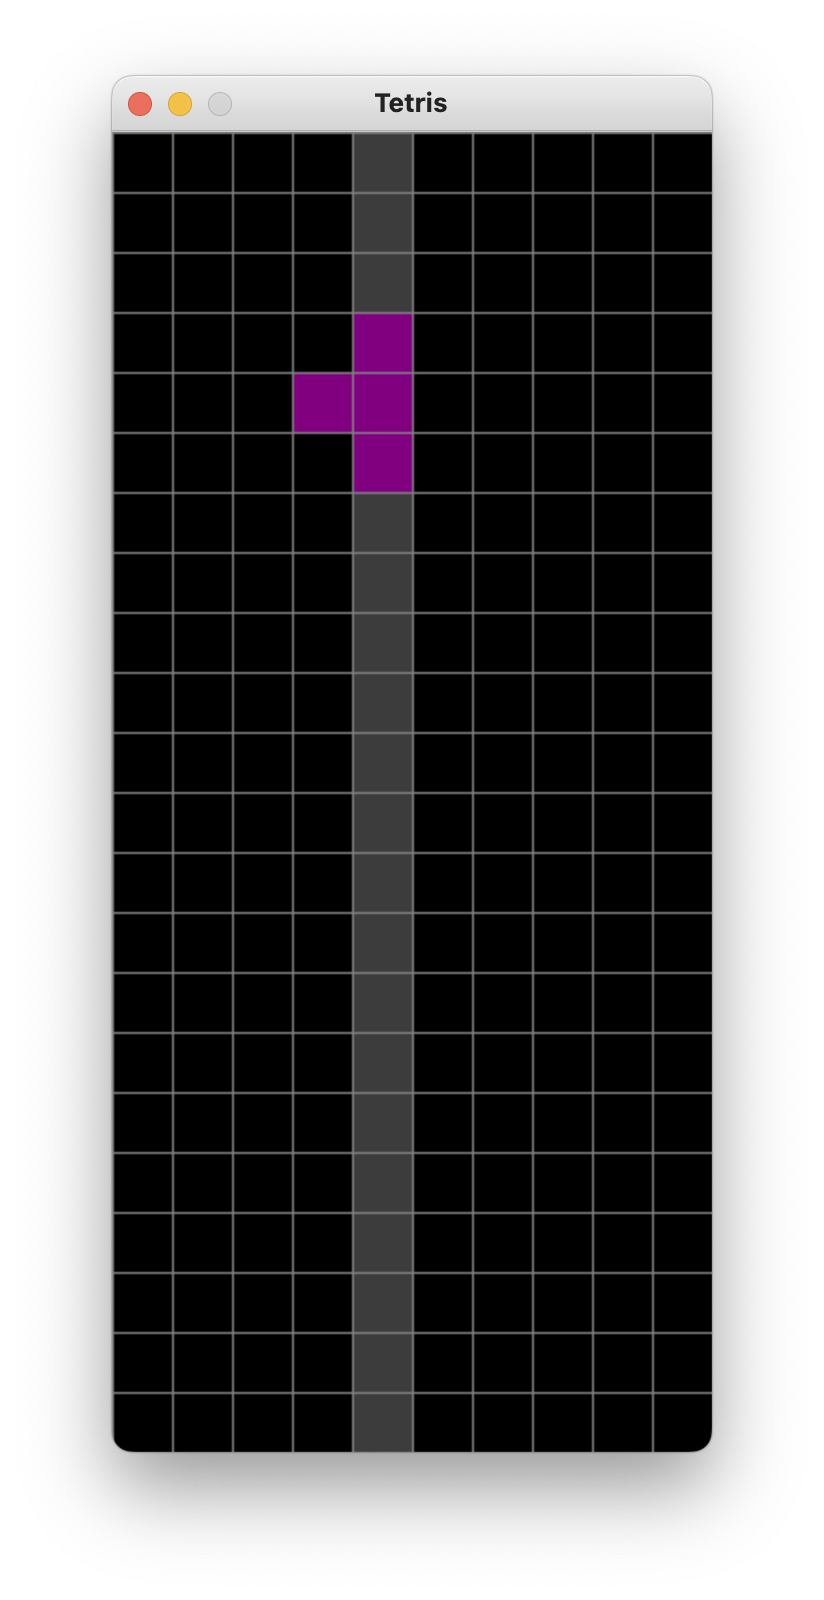
\includegraphics[width=50mm]{images/CH7_4.png}
  \caption{Tブロックの回転}
\end{figure}

回転によりはみ出してしまうことがありますね。これは移動と同じで回転できない状況があるのに、それを検知できずに回転しているからです。

\subsubsection{Q: この教材、いきあたりばったりで作ってないですか?}
多くのメンターさんが共感してくれると思いますが、
基本的にプログラムは一発で動きません。さらに残酷なことに、頑張って書いた時ほど、動かないものです。
ここまできたみなさんには、同じプログラマとして、「せっかく頑張ったのになんでやねん」というこのガッカリ感を
味わってみて欲しいです。

実行する前にこうなることが予期できた人は素晴らしいです。ぜひ、次回以降もこのような予測をしていってください。

\section{回転できるか判定する関数をつくる}
それでは、回転について判定する関数を作ってみましょう。
いくつか方法が考えられますが、今回は、回転した後の座標を計算して、その座標が盤面と衝突しないかどうかを判定する方法を取ります。
\subsection{回転できるか判定する関数をつくる}
以下のように書いてみましょう。戻り値はbool型、すなわちTrueかFalseです。
可能だと分かったらその時点でreturn True、逆に不可能だと分かったらreturn Falseします。
\lstinputlisting[caption={回転できるか判定する関数をつくる}, language=Python]{chapter7/ch7_5_1.py}
ちなみに、もっと賢い方法を思いついた人は、それを書いて試してみましょう。
この教材では直感的な方法をとっています。

次に、\textbf{判定をしてから回転する}部分を作ります。
今回も前回同様に、Boardクラスがブロックの回転する関数を提供します。
\subsection{Boardクラスに回転する関数をつくる}
\lstinputlisting[caption={Boardクラスに回転する関数をつくる}, language=Python]{chapter7/ch7_5_2.py}
これで回転できる時に回転する、機能が完成しました。
最後に、main関数を変更しましょう。
\subsection{main関数を変更する}
\lstinputlisting[caption={main関数を変更する}, language=Python]{chapter7/ch7_5_3.py}
実行すると、Tブロックが正しく回転するようになるはずです。
うまくいかない場合はcan\_rotateが大体間違っていると思うので、先生と相談してください。

\subsubsection{コラム: if \_\_name\_\_ == "\_\_main\_\_"について}
Swimmyの教材には書いていませんが、Pythonには\_\_name\_\_という変数があらかじめ使えます。
もちろん変数なのでprintが可能です。
\begin{lstlisting}[caption=\_\_name\_\_の使い方,language=Python]
print(__name__)
\end{lstlisting}
これを実行すると、\_\_main\_\_と表示されます。これは、このファイルが直接実行されたときに\_\_main\_\_になるということです。
Pythonファイルには、実行する方法が2度あります。
\begin{itemize}
  \item 直接実行する
  \item importして使う
\end{itemize}
importされた時には、\_\_name\_\_はファイル名になります。
import pygameをしたときに
\begin{verbatim}
pygame 2.0.1 (SDL 2.0.14, Python 3.8.3)
Hello from the pygame community. https://www.pygame.org/contribute.html
\end{verbatim}
こんな表示を見たことはありませんか?
おそらく、pygameのファイルにはこんなのが書いてあるはずです
\begin{lstlisting}[caption=pygameのファイルの一部,language=Python]
  print("pygame 2.0.1 (SDL 2.0.14, Python 3.8.3)")
  print("Hello from the pygame community. https://www.pygame.org/contribute.html")
\end{lstlisting}
使い道はかなり限定されていますが、
\begin{itemize}
  \item このファイルが間違ってimportされた時に警告を出したい
  \item importして使って欲しいので直接実行された時はエラーを出したい
  \item バージョンを表示したり、著作権表示をしたい
\end{itemize}
こんな時に使われている傾向があります。
せっかくなので、自分のファイルにも書いてみてください。
\lstinputlisting[language=Python]{chapter7/ch7_5_4.py}
import tetrisのあたりでprintが実行され、自分の名前が出てくるはずです。

\section{まとめ}
今回はTブロックを作りました。TブロックはOブロックと違い、回転が必要なブロックです。
そのため、回転できるかどうかを判定する機能を追加しました。

\chapter{他のブロックを作る}
\section{LBlockクラス}
今までのTブロックを元に、Lブロックを作ります。
\begin{figure}[h]
  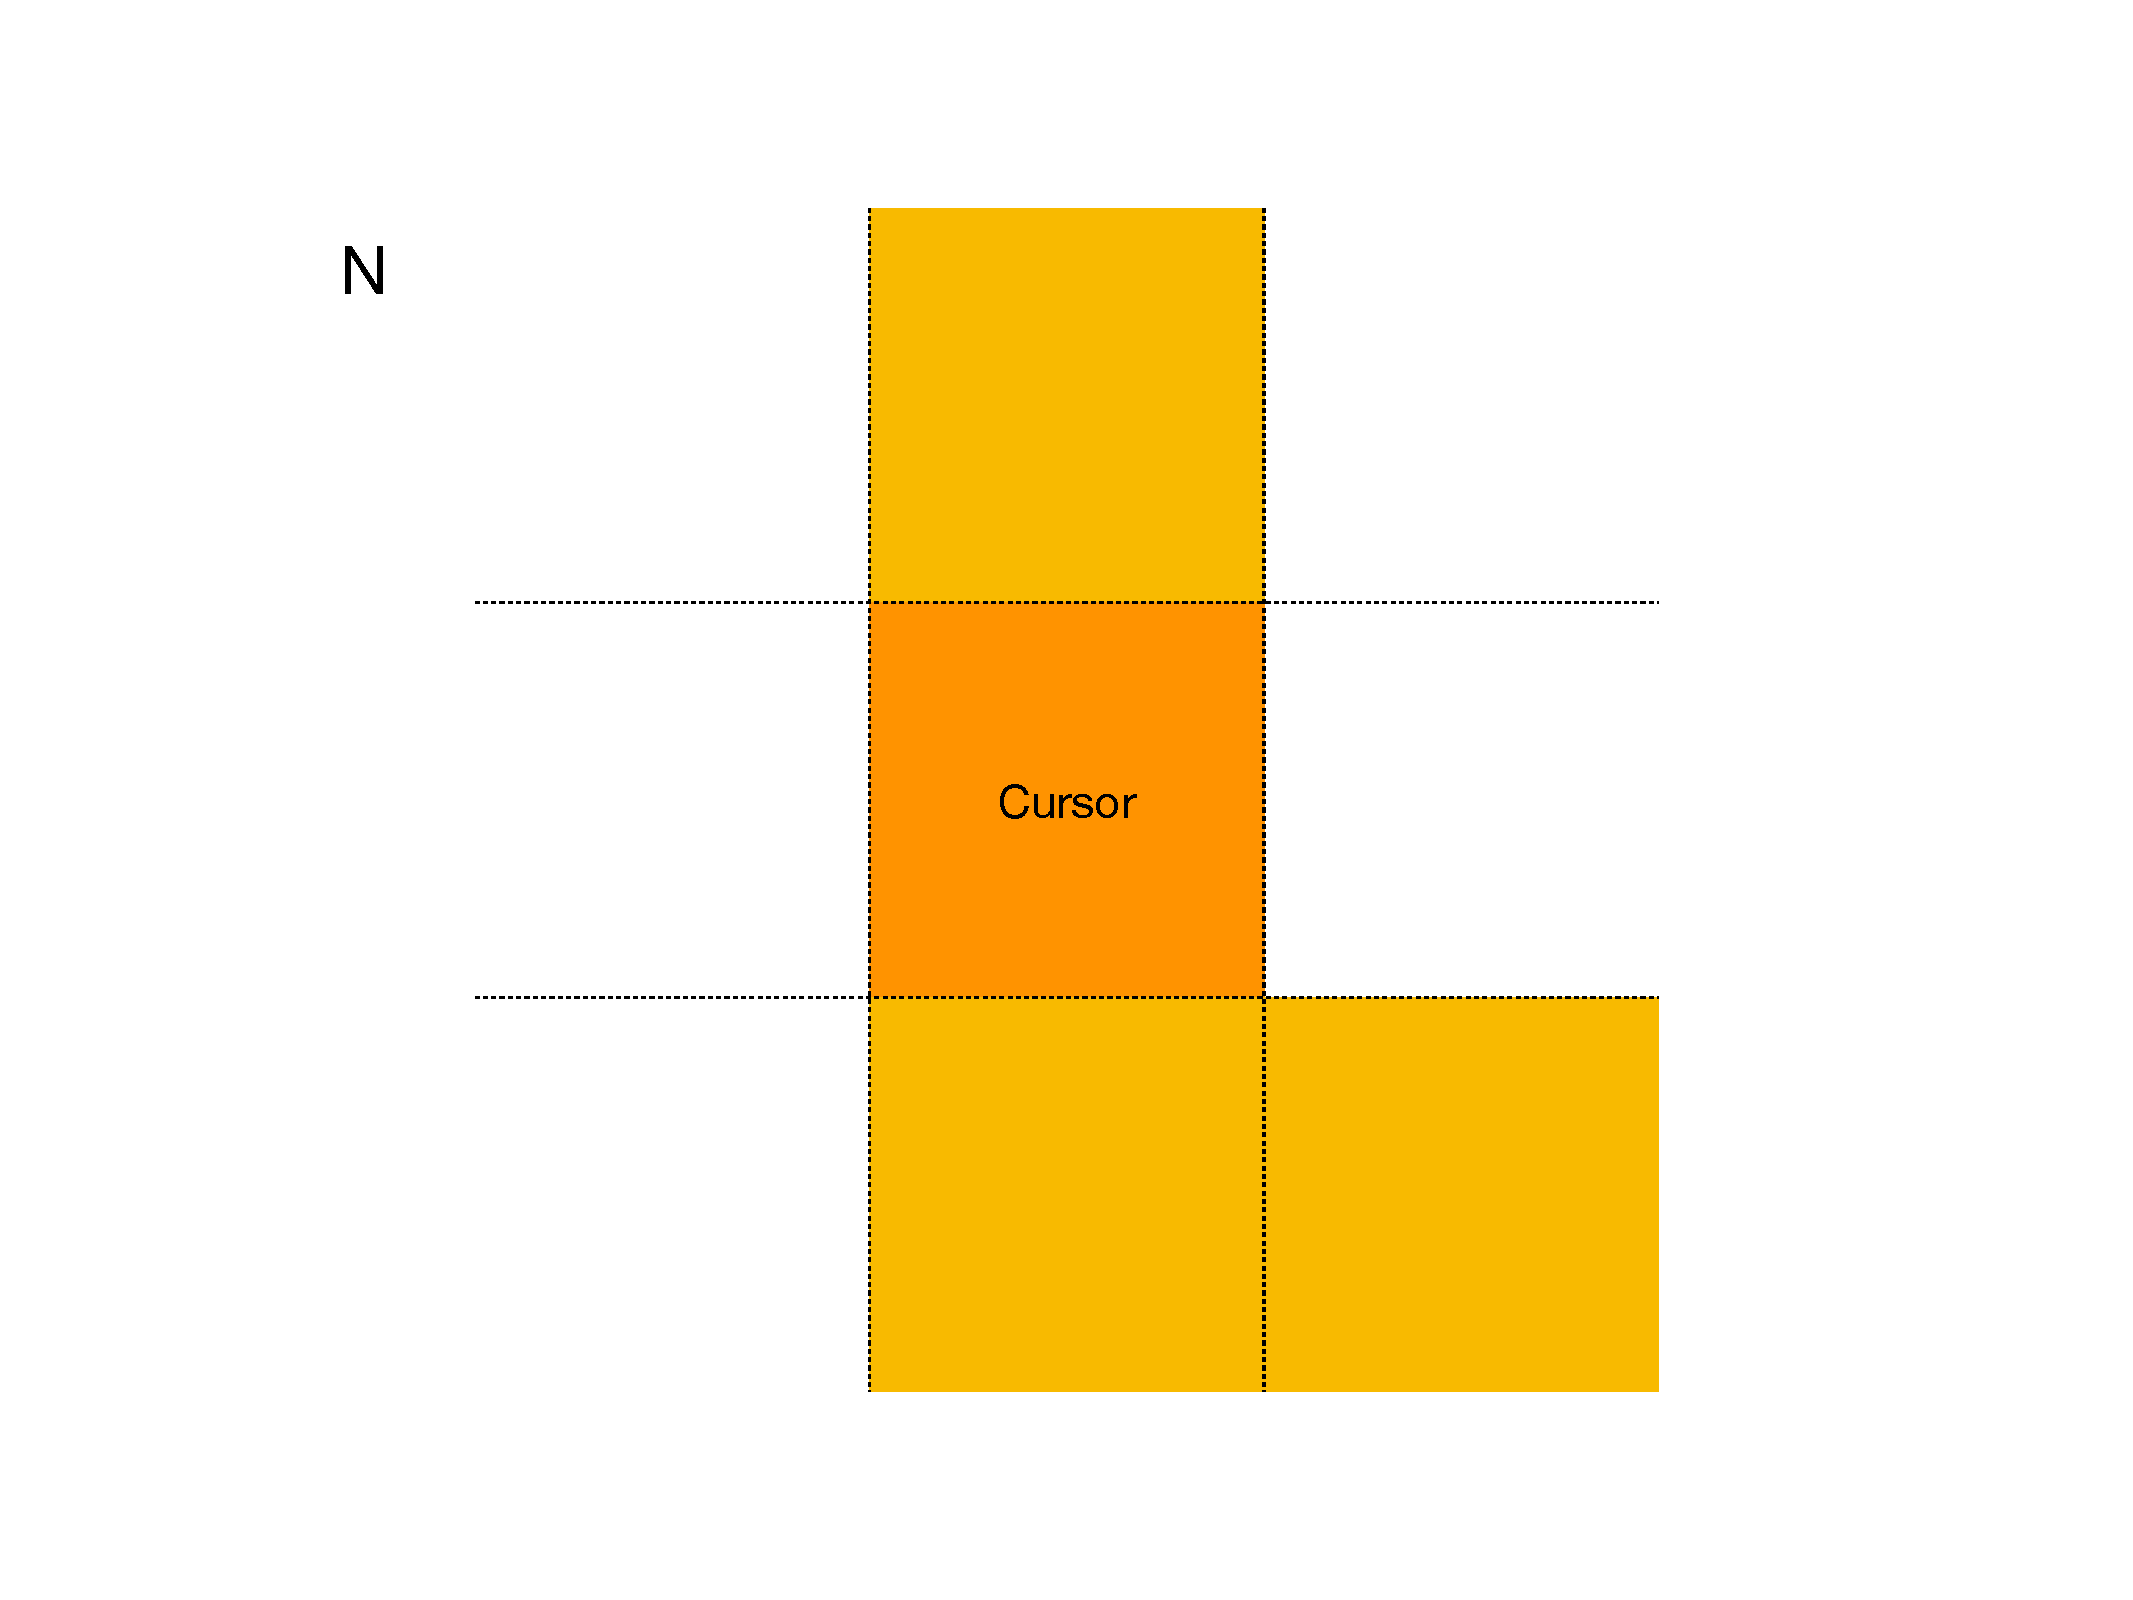
\includegraphics[width=60mm, page=1]{images/LBlock.pdf}
  \includegraphics[width=60mm, page=2]{images/LBlock.pdf}
  \includegraphics[width=60mm, page=3]{images/LBlock.pdf}
  \includegraphics[width=60mm, page=4]{images/LBlock.pdf}
  \caption{Lブロック}
\end{figure}
クラス名はLBlockとしましょう。色はオレンジが多いようです。
以下の関数を作るのを忘れないでください。
\begin{itemize}
  \item block\_info関数 ... カーソルの位置から自分のブロックの様子を座標のリストで返します。
  \item rotate関数 ... 回転します。回転できるかは気にせず、とりあえずselfに入っているrotationという変数を変えるだけにします。
  \item can\_rotate関数 ... 実際に回転したときにはみ出さないか、他のブロックとぶつからないか判定します。引数cursorで現在の位置を、引数board\_infoで盤面の情報を取得します。
  \item can\_go\_up関数 ... 上に移動できるか判定します。引数cursorで現在の位置を、引数board\_infoで盤面の情報を取得します。
  \item can\_go\_down関数 ... 下に移動できるか判定します。引数cursorで現在の位置を、引数board\_infoで盤面の情報を取得します。
  \item can\_go\_right関数 ... 右に移動できるか判定します。引数cursorで現在の位置を、引数board\_infoで盤面の情報を取得します。
  \item can\_go\_left関数 ... 左に移動できるか判定します。引数cursorで現在の位置を、引数board\_infoで盤面の情報を取得します。
\end{itemize}
出来上がったら、main関数で表示してみましょう。
main.pyのmoving\_block = の部分を変更したらできるはずです。

\section{JBlockクラス}
次にJブロックを作ります。
\begin{figure}[h]
  \includegraphics[width=60mm, page=9]{images/Blocks.pdf}
  \includegraphics[width=60mm, page=10]{images/Blocks.pdf}
  \includegraphics[width=60mm, page=11]{images/Blocks.pdf}
  \includegraphics[width=60mm, page=12]{images/Blocks.pdf}
  \caption{Jブロック}
\end{figure}
関数も同じものを作ります。
自分を信じすぎず、一つブロックを作ったらきちんと表示、回転、移動ができるか確認しましょう。

\newpage
\section{SBlockクラス}
次にSブロックを作ります。
\begin{figure}[h]
  \includegraphics[width=60mm, page=13]{images/Blocks.pdf}
  \includegraphics[width=60mm, page=14]{images/Blocks.pdf}
  \includegraphics[width=60mm, page=15]{images/Blocks.pdf}
  \includegraphics[width=60mm, page=16]{images/Blocks.pdf}
  \caption{Sブロック}

\end{figure}
関数も同じものを作ります。

\newpage
\section{ZBlockクラス}
次にZブロックを作ります。
\begin{figure}[h]
  \includegraphics[width=60mm, page=17]{images/Blocks.pdf}
  \includegraphics[width=60mm, page=18]{images/Blocks.pdf}
  \includegraphics[width=60mm, page=19]{images/Blocks.pdf}
  \includegraphics[width=60mm, page=20]{images/Blocks.pdf}
  \caption{Zブロック}
\end{figure}

\newpage
\section{IBlockクラス}
最後にIブロックを作ります。
\begin{figure}[h]
  \includegraphics[width=60mm, page=21]{images/Blocks.pdf}
  \includegraphics[width=60mm, page=22]{images/Blocks.pdf}
  \includegraphics[width=60mm, page=23]{images/Blocks.pdf}
  \includegraphics[width=60mm, page=24]{images/Blocks.pdf}
  \caption{Iブロック}
\end{figure}
うまく動いていることが確認できたでしょうか。
ブロックはこれで全てです。お疲れ様でした。


\chapter{ブロックの落下とランダムなブロックの生成}
\section{ブロックの落下}
今までのプログラムでは、ブロックが動くのはキー入力を受け取ったときだけでした。
しかし、テトリスでは一定時間ごとにブロックが落ちてくるようになっています。
今回は1秒に一度ブロックが落ちるようにしましょう。
\subsection{1秒ごとに落とす}
1秒を測るためには、時間を計測する必要があります。
今回、main関数のwhile文は一秒間に60回実行されています。
つまり、1秒を測るためには60回のループを数えればいいということです。
\lstinputlisting[caption={main関数を変更する}, language=Python]{chapter9/ch9_1_1.py}
これを実行すると、1秒ごとにブロックが落ちていくようになります。

\subsection{ブロックを落とす}
Boardクラスにdrop関数を追加します。
dropとは、落とす、こぼす、という意味があります。
落ちれなくなるところまで落とすという関数です。
\lstinputlisting[caption={Boardクラスにdrop関数を追加する}, language=Python]{chapter9/ch9_1_2.py}
また、main関数を変更して、スペースキーでブロックを落とせるようにします。
\lstinputlisting[caption={main関数を変更する}, language=Python]{chapter9/ch9_1_3.py}
きちんと動いているでしょうか。

\section{ランダムなブロックの生成}
今度はランダムにブロックを生成する機能を追加します。
generate\_block関数を作り、その中でランダムにブロックを生成するようにします\footnote{generate: 生成する}。
その関数は\_\_init\_\_関数の中で呼び出すと、最初のブロックがランダムになります。
\lstinputlisting[caption={ランダムなブロックの生成}, language=Python]{chapter9/ch9_2_1.py}
これで、ランダムなブロックが生成されるようになりました。
mainでブロックを設定する必要がなくなったので、消してしまいましょう。
\lstinputlisting[caption={main関数の変更}, language=Python]{chapter9/ch9_2_2.py}
これで、ランダムなブロックが生成されるようになりました。
しかし、ブロックが一番下まで落ちても、次のブロックに切り替わりません。
次の章でその機能を追加します。

\chapter{次のブロックへ切り替える}
\section{ブロックが一番下まで落ちた時とは}
ブロックがこれ以上下に落ちられないとき、次のブロックに切り替える処理を書きます。
現在、1秒に一回、ブロックが落ちるようになっているので、そこを利用しましょう。
\begin{figure}[h]
  \centering
  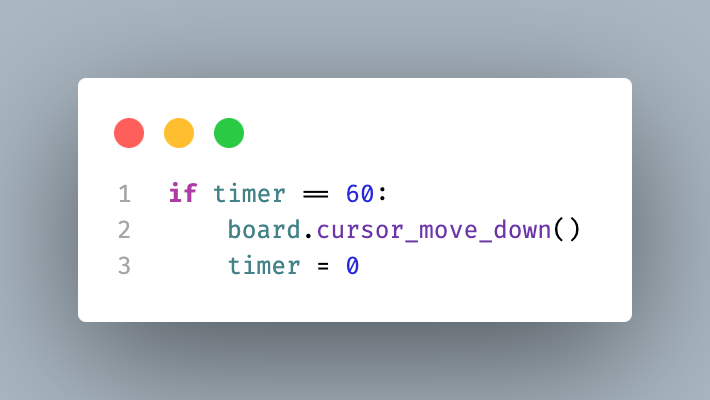
\includegraphics[width=100mm]{images/timer.png}
  \caption{「一秒経った時」を実現しているif文}
\end{figure}

\subsection{Boardクラスに新しい関数updateを追加}
Boardクラスに新しい関数updateを追加します。
mainに「もしブロックが…」のような処理を書いても動きはするのですが、
役割分担の考え方からBoardクラスに書くことにします。
\lstinputlisting[caption={定期的にブロックを落とし、落とせないなら次のブロックを用意するupdate関数}, language=Python]{chapter10/ch10_1_1.py}
次に、main関数を変更します。今まで単純にブロックを落としていた部分をupdate関数に変更します。
\lstinputlisting[caption={main関数を変更する}, language=Python]{chapter10/ch10_1_2.py}
実行すると、ブロックが一番下まで落ちたら次のブロックに切り替わるようになります。

\section{ブロックを積む}
前回のセクションでは、ブロックが切り替わった時に前のブロックが消えてしまう問題がありました。
今回は、ブロックが一番下まで落ちた時に、そのブロックを置く処理を書きます。
\subsection{Boardクラスにfix関数を追加}
Boardクラスにfix関数を追加します\footnote{fix: 固定する、直す}。
ここで、盤面がどのように描かれているかを復習します。
\subsubsection{スクリーンへの書き込みを行なっている場所}
実際にウィンドウへの書き込みを行なっているのは、draw関数です。
その中でも、\textbf{2~5行目が盤面の描画}、7~9行目がカーソルを灰色にする処理、
14~36行目が現在持っているブロックの描画、42~45行目が枠線の描画になっています。
\begin{figure}
  [h]
  \centering
  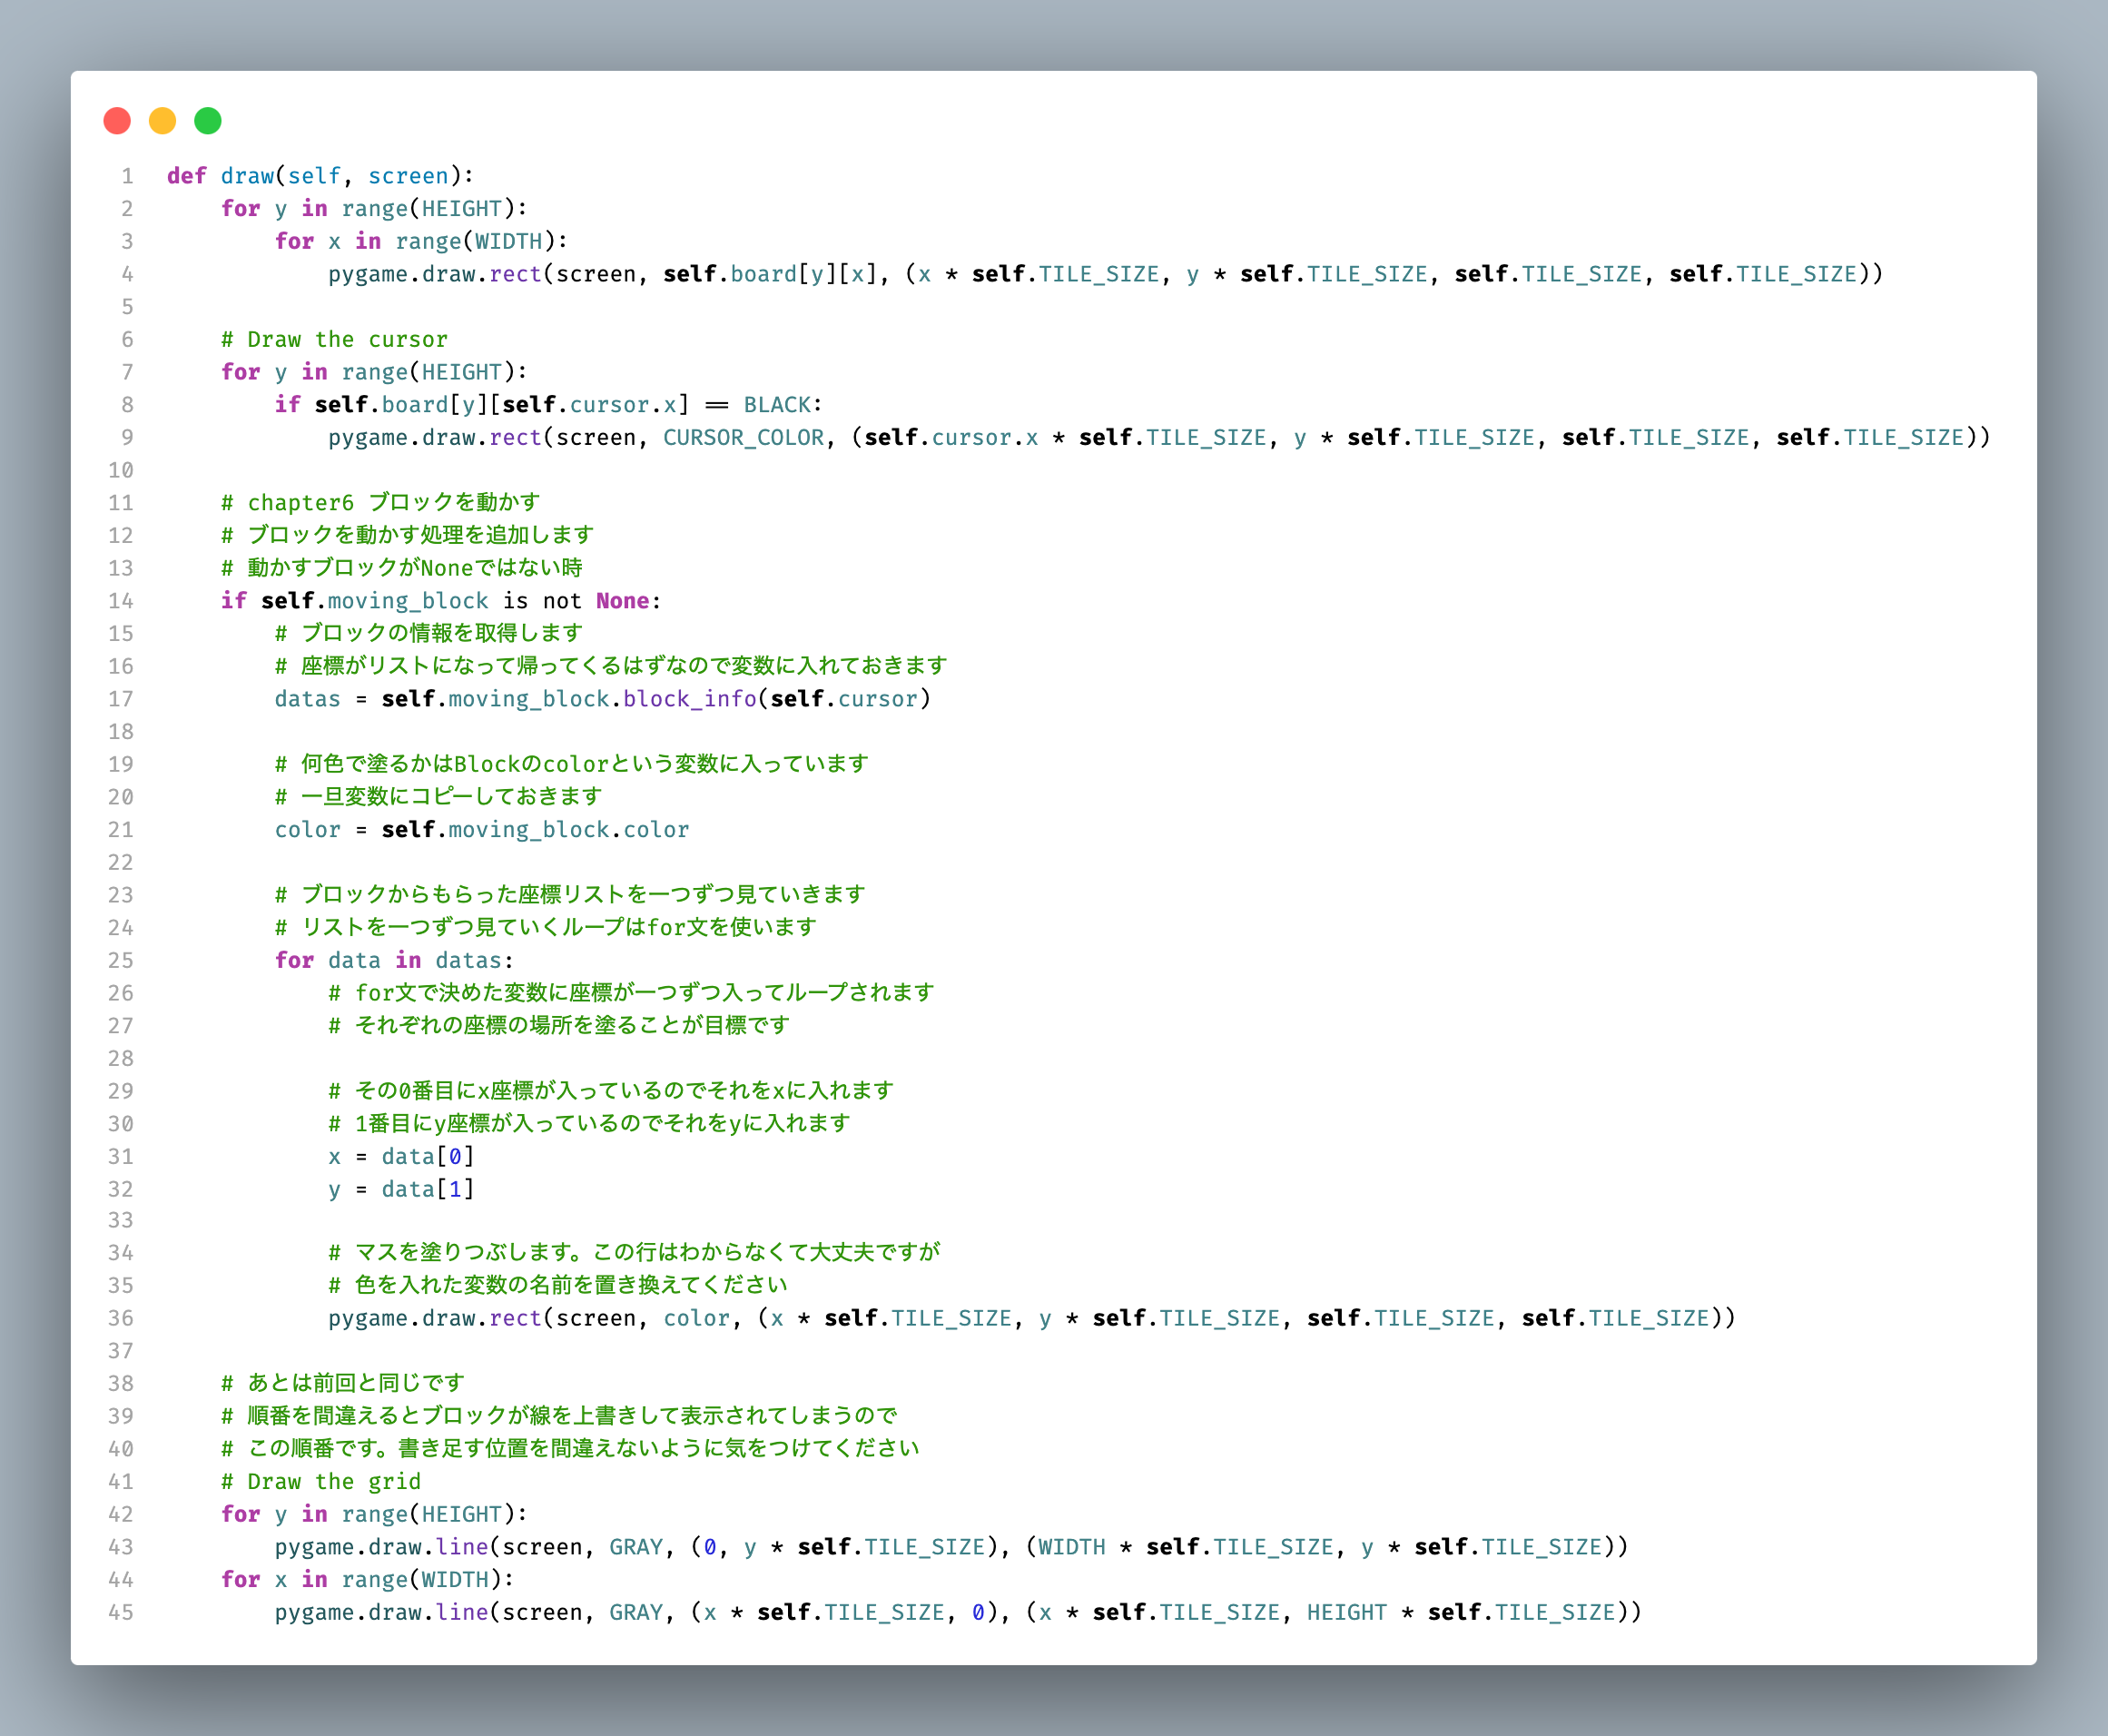
\includegraphics[width=100mm]{images/DrawFunction.png}
  \caption{draw関数の中身}
\end{figure}
ここから、self.boardの中身を変更すれば、draw関数が自動的に画面に反映してくれそうです。
\begin{figure}
  [h]
  \centering
  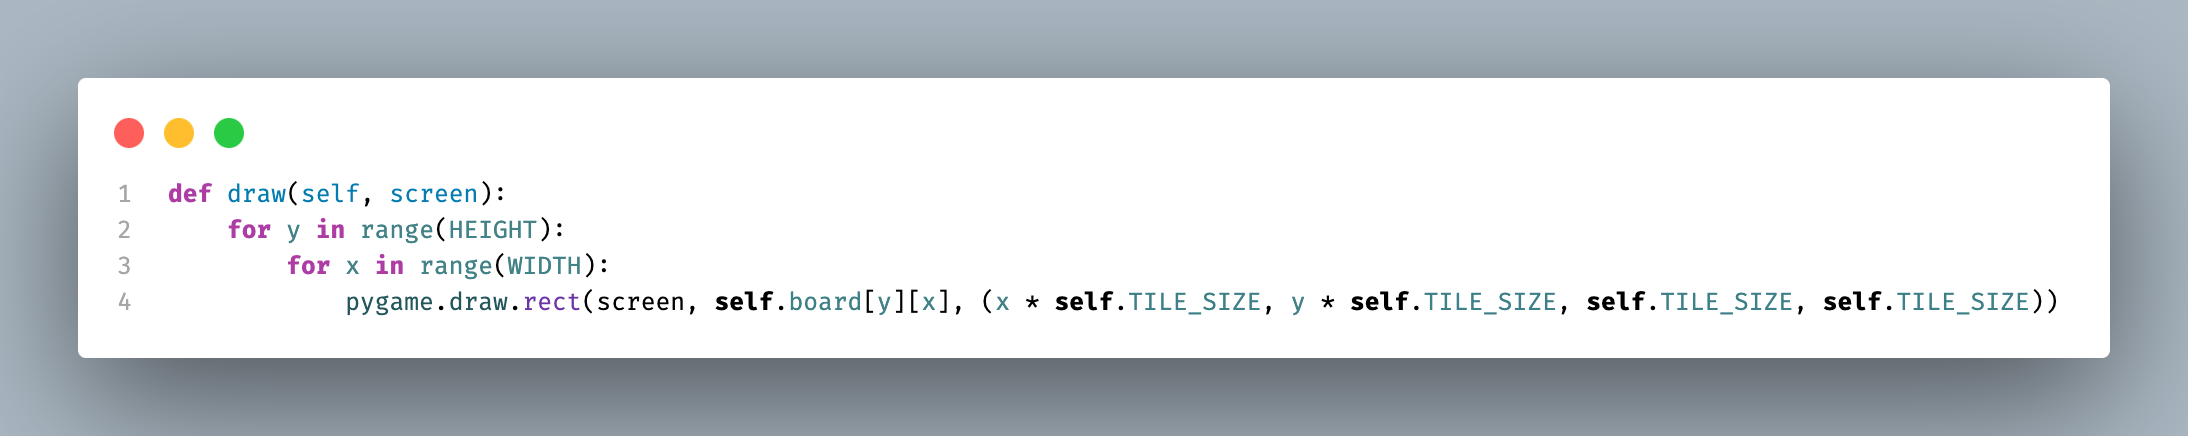
\includegraphics[width=\textwidth]{images/DrawBoard.png}
  \caption{self.boardを変更すれば画面にも反映されそう}
\end{figure}

\subsection{fix関数を実装}
fix関数を実装します。
\lstinputlisting[caption={fix関数}, language=Python]{chapter10/ch10_2_1.py}
次に、update関数を変更します。
\lstinputlisting[caption={update関数を変更}, language=Python]{chapter10/ch10_2_2.py}
実行すると、ブロックが一番下まで落ちたら、そのブロックが盤面に固定されるようになります。

\chapter{行を消す}
\section{盤面を確認して行を消す関数erase\_lines}
盤面を確認して、揃った行を消す関数erase\_linesを作ります。
盤面は、self.boardに2次元配列として保存されています。
配列の配列は下のようなイメージです。

\chapter{自由創作}
ここまでで、基本的なテトリスの作り方を学びました。
残った部分については、自由にアレンジしてみましょう。
\section{自由創作のアイデア}
\begin{itemize}
  \item ゲームオーバーの設定
  \item スコアの計算、表示
  \item スコアに応じた落下速度の変更
  \item 4行消し(Tetris)、Tスピンなどの特殊な消し方の実装
  \item ネクストブロックの表示
  \item ホールド機能の実装
\end{itemize}
このほかにも、自分で考えたアイデアを実装してみましょう。

\section{各プログラムの構成と役割}
自由創作にあたって、各プログラムの構成と役割を確認しておきましょう。
どのプログラムがどのような役割を持っているかを把握することで、具体的にどのプログラムを変更すればよいかがわかります。

\subsection{main関数}
main関数は、ゲーム全体の流れを管理します。
以下のような変数を持っています。
\subsubsection{board変数}
Board型の変数で、盤面、カーソル、保持中のブロックを表します。
\subsubsection{screen変数}
PygameのSurface型の変数で、画面を表します。
\url{https://www.pygame.org/docs/ref/surface.html}に詳しく説明があります。
\subsubsection{clock変数}
Pygameのtime.Clock型の変数で、フレームレートを管理します。
\url{https://www.pygame.org/docs/ref/time.html#pygame.time.Clock}に詳しく説明があります。
\subsubsection{timer変数}
int型の変数で、ゲーム内の一秒を管理するために作りました。
while文の中で1ずつ増やし、60になったら0に戻します。
\begin{figure}
  [h]
  \centering
  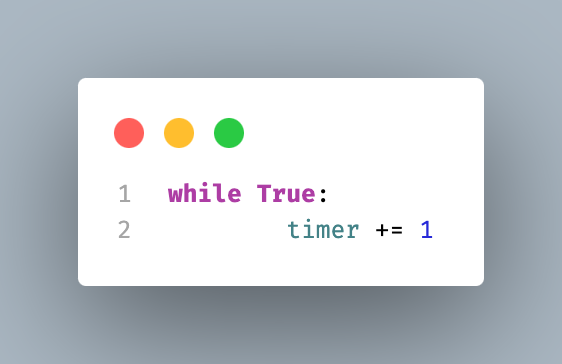
\includegraphics[width=50mm]{images/timerVar.png}
  \caption{timer変数のカウントアップ}
\end{figure}
\begin{figure}
  [h]
  \centering
  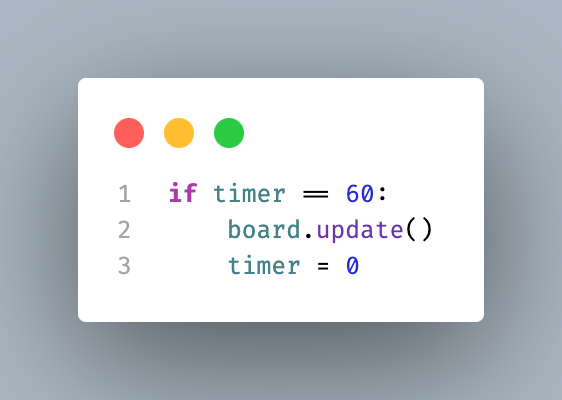
\includegraphics[width=50mm]{images/timerReset.png}
  \caption{timer変数のリセット}
\end{figure}
boardのupdate関数を呼び出しているのもここです。
ブロックの落下のタイミングを早くしたい場合は、60の部分を変数を用いたり、別の値にすると変化します。
\subsubsection{main関数の中のwhile文}
while文の中で、盤面を更新します。
また、キー入力を受け取り、board変数の関数を呼び出します。

\subsection{Boardクラス}
\subsubsection{\_\_init\_\_関数}
以下の変数を初期化します。
\begin{itemize}
  \item board変数 \newline 2次元リストで盤面を表します。中身にはブロックの色を入れています。board[y][x]で(x,y)の座標の色を取得できます。
  \item TILE\_SIZE変数 \newline マスのサイズを表します。大きくすると盤面が大きくなります。
  \item cursor変数
\end{itemize}
最後に、generate\_block関数を呼び出すことで、moving\_block変数も初期化しています。
holding\_block変数を追加すれば、ホールド機能を実装することもできます。
\subsubsection{draw関数}
保持しているboard変数を元に、盤面を描画します。
次に、cursor変数を元に、保持中のブロックとカーソルを描画します。
枠線も描画しています。

\subsubsection{window\_size関数}
ブロックのサイズを元に、ウィンドウのサイズを計算します。
pygame.display.set\_mode関数でウィンドウを作成する際に使うことを想定しています。

\subsubsection{cursor\_move\_up,down,left,right関数}
カーソルを動かす関数です。そのままcursorの関数を呼び出しています。
盤面端の判定などはCursorクラスで行なっています。

\subsubsection{block\_rotate関数}
ブロックを回転させる関数です。moving\_block変数を用いて回転の判定、実際の回転を行います。

\subsubsection{drop関数}
while文を用いて、ブロックを落下させる関数です。

\subsubsection{update関数}
main関数からtimer変数の更新関連で呼び出される関数です。
一マス落下させる処理や、一番下まで落ちた際にはブロックを固定するfix関数や、
次のblockを生成するgenerate\_block関数の呼び出し、最後に行を消去するerase\_lines関数の呼び出しを行います。

\subsubsection{fix関数}
ブロックを固定する関数です。ブロックの色をboard変数に書き込みます。
ブロックの固定先が盤面から出てしまった場合、ゲームオーバーとすることも可能です。

\subsubsection{generate\_block関数}
次のブロックを生成する関数です。カーソルの位置を上に戻した後、次のブロックをランダムに生成し、moving\_block変数に代入します。
このタイミングで、次のブロックを表示するために、next\_block変数を作成して代入すれば、次のブロックを表示することもできるかもしれません。

\subsubsection{erase\_lines関数}
行を消去する関数です。BLACKが含まれていない行を消去します。
行を消去したら、上から空の行を追加することで、盤面全体の行数が変わらないようにしています。
この際、カウンターとなる変数を用意して行を消すたびにカウンターを増やし、4だったらTetrisとすれば、Tetrisの処理を行うこともできます。
さらに、スコア変数をBoardクラス全体で持っていれば、スコアの計算も行うことができます。

\subsection{各Blockクラス}
\subsubsection{\_\_init\_\_関数}
各ブロックの色や向きを初期化します。
color変数やrotation変数を持っています。

\subsubsection{block\_info関数}
各ブロックの形を返す関数です。各ブロックの形を座標のリストで返します。
ブロックの現在位置を知るために、Cursor型の変数を引数にとります。

\subsubsection{can\_go\_up,down,left,right関数}
ブロックが移動できるかどうかを判定する関数です。
移動できる場合はTrue、できない場合はFalseを返します。
自分の位置を知るために、Cursor型の変数を引数にとり、
まわりのブロックの情報を知るためにBoard型の変数を引数にとります。

\subsubsection{can\_rotate関数}
ブロックが回転できるかどうかを判定する関数です。
回転できる場合はTrue、できない場合はFalseを返します。
自分の位置を知るために、Cursor型の変数を引数にとり、
まわりのブロックの情報を知るためにBoard型の変数を引数にとります。

\subsubsection{rotate関数}
ブロックを回転させる関数です。
実際にはrotation変数を変更しているだけで、
そのrotation変数を元にblock\_info関数で回転後の形を計算し
その値をBoardが描画し画面に反映させています。

\subsection{Cursorクラス}
\subsubsection{\_\_init\_\_関数}
カーソルの位置を初期化します。
x変数、y変数を持っています。

\subsubsection{move\_up,down,left,right関数}
カーソルを動かす関数です。
引数として取ったblockに移動可能かどうかを判定してもらい、
移動可能な場合はカーソルを移動させます。

\section{最後に}
ここまでのプログラミングで作ったクラスは以下のような関係になっています。
\begin{figure}
  [h]
  \centering
  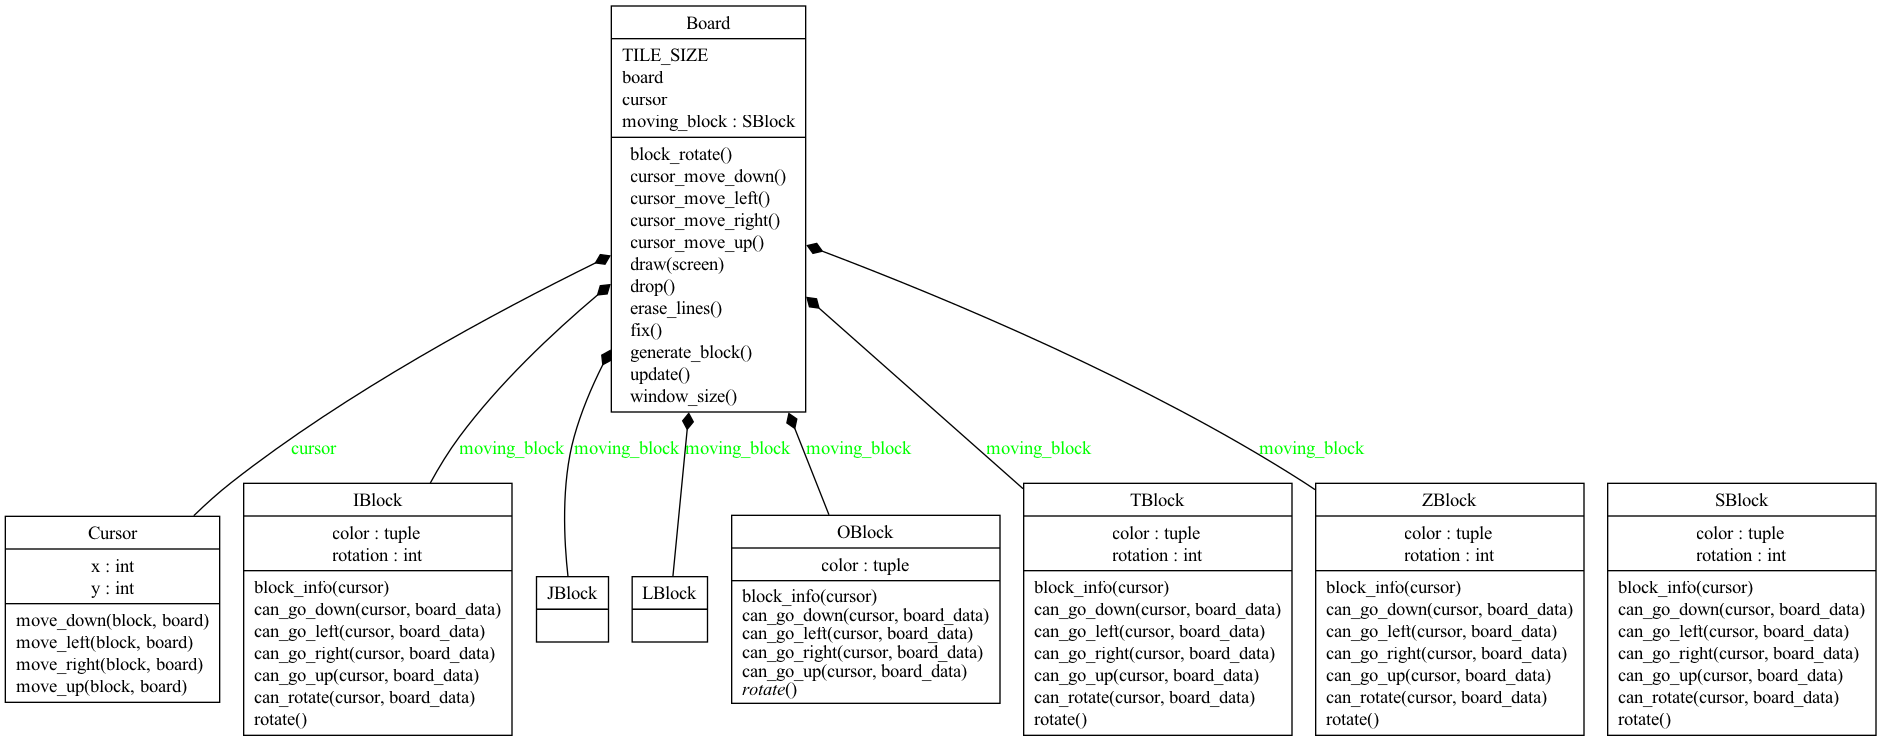
\includegraphics[width=\textwidth]{images/classes_tetris.png}
  \caption{クラス図}
\end{figure}
このような図をクラス図といいます。
\newpage
Pythonに限らず、オブジェクト指向プログラミングではこのように
クラスを作り、機能を整理し、その連携をデザインすることでプロジェクトを進めていきます。
例えば、ChromiumというGoogle Chromeなどの元となるブラウザの一部は、以下のようなクラス図を持っています。
\footnote{\url{https://www.chromium.org/developers/class-diagram-webkit-webcore-to-chrome-browser/}より引用。}
\begin{figure}
  [h]
  \centering
  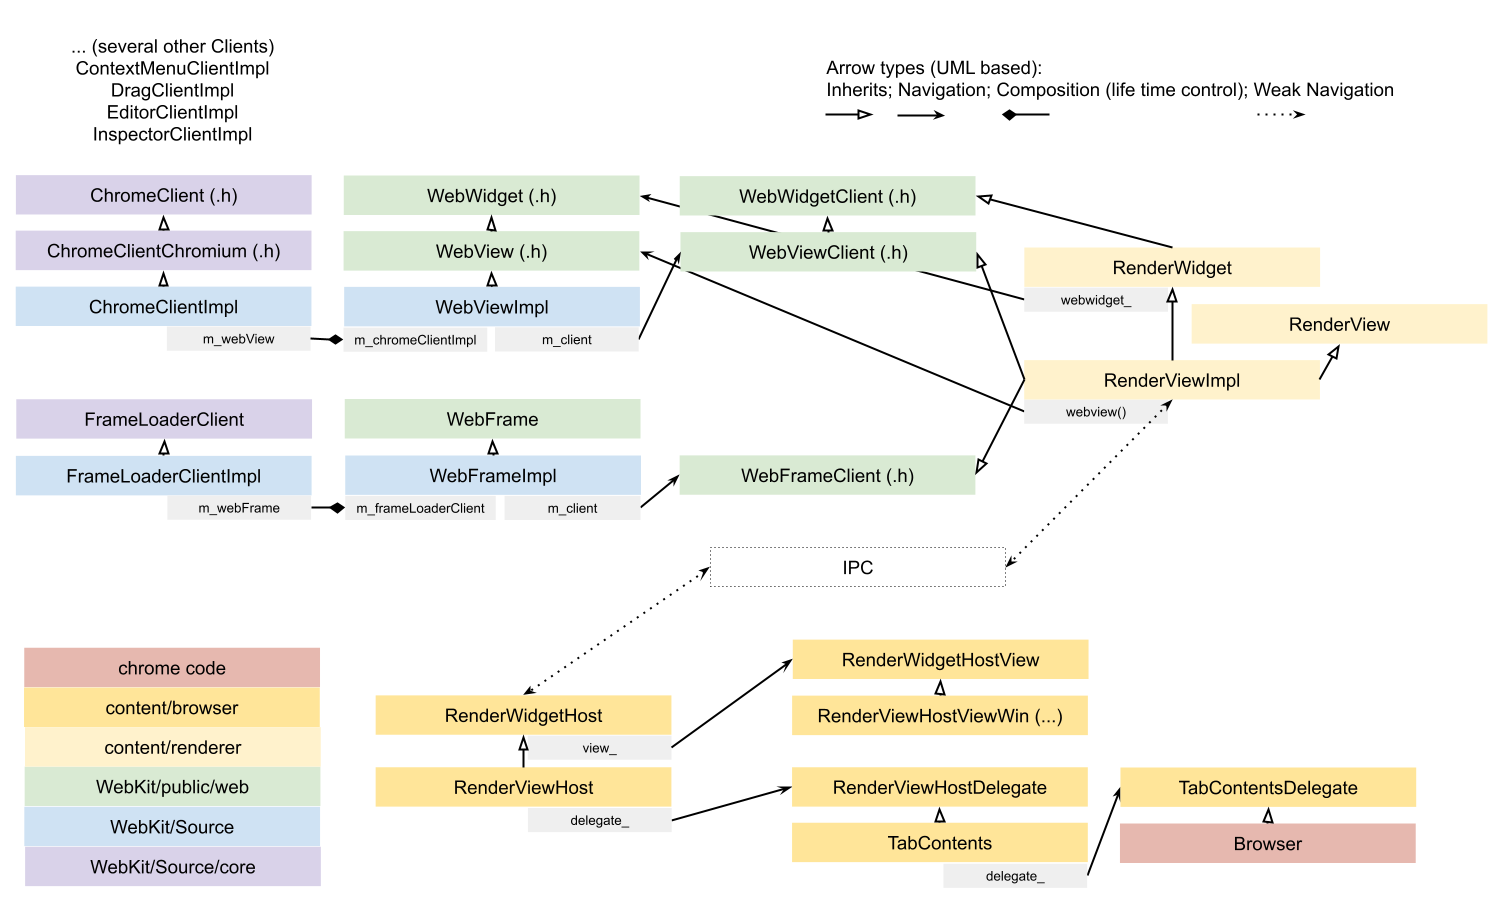
\includegraphics[width=\textwidth]{images/Chromium.png}
  \caption{Chromiumのクラス図(一部)}
\end{figure}
今回作ったものよりも複雑で、多くのクラスが連携してWebブラウザという高機能なプログラムを作っています。
しかし、簡単な機能を持ったクラスをひとつひとつ組み合わせて作っていくという考え方は同じです。

これからプログラマーになるにあたって、クラスを設計するという機会は必ずあると思います。
ぜひ、この経験を活かして自分のプログラムをより良いものにしていってください。

\end{document}